%-------------------------------------------------------------------------------
% Three-way TCRE electrolyte comparison: Felt vs Gel vs Paste
% Target journal: MDPI Sensors
%
% Compile mode toggle:
%   \previewtrue   -> compile WITHOUT the MDPI template (default; works on
%                     vanilla TeX Live / Overleaf, no template upload needed).
%                     Layout mimics MDPI Sensors but is not the official class.
%   \previewfalse  -> compile WITH the official MDPI Sensors template.
%                     Requires Definitions/mdpi.{cls,bst,cfg} from
%                       https://www.mdpi.com/authors/latex
%                     Place the Definitions/ folder next to this file, then flip
%                     the toggle below to \previewfalse.
%
% Build:  pdflatex main && bibtex main && pdflatex main && pdflatex main
%-------------------------------------------------------------------------------

\newif\ifpreview
\previewtrue   % <-- flip to \previewfalse once Definitions/mdpi.cls is uploaded

\ifpreview
%======================== PREVIEW (no MDPI template) ===========================
\documentclass[10pt,a4paper]{article}
\usepackage[margin=2.5cm]{geometry}
\usepackage[utf8]{inputenc}
\usepackage[T1]{fontenc}
\usepackage{lmodern}
\usepackage{amsmath,amssymb,amsfonts}
\usepackage{graphicx}
\usepackage{booktabs}
\usepackage{array}
\usepackage{xcolor}
\usepackage{hyperref}
\usepackage{enumitem}
\usepackage{caption}
\usepackage{subcaption}
\usepackage{float}
\usepackage{titlesec}
\usepackage{authblk}
\usepackage{textgreek}
\providecommand{\upmu}{\ensuremath{\mu}}        % \upmu fallback for V/bit (works in math+text)
\hypersetup{colorlinks=true, linkcolor=black, citecolor=blue, urlcolor=blue}
\setlist[itemize]{leftmargin=1.4em, itemsep=2pt, topsep=4pt}
\setlist[enumerate]{leftmargin=1.6em, itemsep=2pt, topsep=4pt}
\titleformat*{\section}{\Large\bfseries}
\titleformat*{\subsection}{\large\bfseries}

% MDPI-only commands become no-ops in preview mode so the body compiles unchanged.
\newcommand{\Title}[1]{\title{#1}}
\newcommand{\TitleCitation}[1]{}
\newcommand{\Author}[1]{\author{#1}}
\newcommand{\AuthorNames}[1]{}
\newcommand{\AuthorCitation}[1]{}
\newcommand{\address}[1]{}
\newcommand{\corres}[1]{\gdef\PreviewCorres{#1}}
\newcommand{\PreviewCorres}{}
\renewcommand{\abstract}[1]{\gdef\PreviewAbstract{#1}}
\newcommand{\PreviewAbstract}{}
\newcommand{\keyword}[1]{\gdef\PreviewKeywords{#1}}
\newcommand{\PreviewKeywords}{}
\newcommand{\firstpage}[1]{}
\newcommand{\pubvolume}[1]{}
\newcommand{\issuenum}[1]{}
\newcommand{\articlenumber}[1]{}
\newcommand{\pubyear}[1]{}
\newcommand{\copyrightyear}[1]{}
\newcommand{\externaleditor}[1]{}
\newcommand{\datereceived}[1]{}
\newcommand{\daterevised}[1]{}
\newcommand{\dateaccepted}[1]{}
\newcommand{\datepublished}[1]{}
\newcommand{\hreflink}[1]{}
\newcommand{\orcidA}{}
\newcommand{\orcidB}{}
\newcommand{\orcidC}{}
\newcommand{\orcidD}{}
\newcommand{\authorcontributions}[1]{\section*{Author Contributions}#1}
\newcommand{\funding}[1]{\section*{Funding}#1}
\newcommand{\institutionalreview}[1]{\section*{Institutional Review Board Statement}#1}
\newcommand{\informedconsent}[1]{\section*{Informed Consent Statement}#1}
\newcommand{\dataavailability}[1]{\section*{Data Availability Statement}#1}
\newcommand{\acknowledgments}[1]{\section*{Acknowledgments}#1}
\newcommand{\conflictsofinterest}[1]{\section*{Conflicts of Interest}#1}
\newcommand{\reftitle}[1]{\renewcommand{\refname}{#1}}
\newcommand{\externalbibliography}[1]{}
\newcommand{\printendnotes}[1][]{}
\newenvironment{adjustwidth}[2]{}{}
\providecommand{\extralength}{0pt}
\else
%======================== OFFICIAL MDPI Sensors template =======================
\documentclass[sensors,article,submit,pdftex,moreauthors]{Definitions/mdpi}
\firstpage{1}
\makeatletter
\setcounter{page}{\@firstpage}
\makeatother
\pubvolume{1}
\issuenum{1}
\articlenumber{0}
\pubyear{2026}
\copyrightyear{2026}
\externaleditor{Academic Editor: }
\datereceived{}
\daterevised{}
\dateaccepted{}
\datepublished{}
\hreflink{https://doi.org/}
\fi
%==============================================================================

% Collaborator markup (works in either mode).
\usepackage{xcolor}
\newcommand{\TBD}[1]{{\color{red}\textbf{[TBD: #1]}}}
\newcommand{\NOTE}[1]{{\color{blue}\textit{[note: #1]}}}

\Title{A Methods-Harmonized Comparison of Tripolar Concentric Ring Electrode Constructions for Non-Invasive EEG: Saline-Soaked Felt, Conductive Gel, and Paste}

\TitleCitation{A methods-harmonized comparison of tripolar concentric ring electrode constructions for non-invasive EEG}

\newcommand{\orcidauthorA}{0000-0000-0000-0000}
\newcommand{\orcidauthorB}{0000-0000-0000-0000}
\newcommand{\orcidauthorC}{0000-0000-0000-0000}
\newcommand{\orcidauthorD}{0000-0000-0000-0000}

\Author{Shayan Khodabakhsh $^{1,}$*\orcidA{}, Behtom Adeli $^{1}$\orcidB{}, Maryam \TBD{Surname} $^{1}$\orcidC{}, and Walter G. Besio $^{1}$\orcidD{}}

\AuthorNames{Shayan Khodabakhsh, Behtom Adeli, Maryam \TBD{Surname}, and Walter G. Besio}

\AuthorCitation{Khodabakhsh, S.; Adeli, B.; \TBD{Maryam Surname}; Besio, W.G.}

\address{%
$^{1}$ \quad Department of Electrical, Computer and Biomedical Engineering, University of Rhode Island, Kingston, RI, USA; \TBD{co-author emails}
}

\corres{Correspondence: skhodabakhsh@uri.edu}

%-------------------------------------------------------------------------------
\abstract{Tripolar concentric ring electrodes (TCREs) provide an on-board surface-Laplacian derivation (tEEG) alongside a conventional outer-ring recording (eEEG). Published TCRE studies use different constructions---saline-soaked felt, conductive gel, paste---and different processing pipelines, which makes cross-study comparisons difficult. We report a pilot, methods-harmonized comparison of three TCRE constructions across two acquisition setups: a saline-soaked-felt setup ($n=10$), a conductive-gel setup ($n=13$), and a paste TCRE present in both setups as a cross-setup bridge. Both setups use the same hardware Laplacian on TCREs of identical ring geometry, so the cross-construction contrast is on electrolyte and coupling rather than on the Laplacian estimator. All recordings pass through a single minimal pipeline (60~Hz notch; zero-phase FIR 0.05--55~Hz bandpass) and are evaluated on scale-invariant endpoints: alpha-band SNR, eyes-closed/eyes-open reactivity, and tEEG--eEEG spectrogram SSIM. The Berger effect is detected on Paste tEEG in 21/23, Gel tEEG in 13/13, and Felt tEEG in 10/10 subjects. tEEG--eEEG SSIM shows a strong construction effect (Felt $0.31 <$ Gel $0.52 <$ Paste $0.71$; Felt-tEEG vs.\ Gel-tEEG $U=0$, $p<0.001$, $d=-2.52$). The paste-TCRE bridge yields no detected between-setup differences. Conclusions are descriptive given the pilot-scale cohort.}

\keyword{tripolar concentric ring electrode; surface Laplacian; EEG; alpha rhythm; visual evoked potential; methods harmonization; electrolyte; signal quality}

\begin{document}

\ifpreview
% In preview mode we render the title block, abstract, and keywords manually,
% since the MDPI commands above were captured as no-ops or stored macros.
\maketitle
\begin{center}\small\PreviewCorres\end{center}
\begin{center}
\begin{minipage}{0.9\linewidth}
\noindent\textbf{Abstract.} \PreviewAbstract\par\medskip
\noindent\textbf{Keywords:} \PreviewKeywords
\end{minipage}
\end{center}
\medskip
\hrule
\medskip
\fi

%-------------------------------------------------------------------------------
\section{Introduction}

The tripolar concentric ring electrode (TCRE) places three concentric conductive rings at a single scalp site and produces two simultaneous derivations: an outer-ring conventional recording (eEEG) referenced to a remote site, and an on-board surface-Laplacian estimate computed from all three rings (tEEG)~\cite{besio2006}. The Laplacian acts as a spatial high-pass filter and has been shown to suppress volume conduction, sharpen focal source detection, and reduce reference-related artifact relative to disc EEG~\cite{besio2006,koka2007}.

A practical question for any TCRE study is how the device couples to the scalp. Three constructions are commonly used: saline-soaked felt pads, conductive gel, and conductive paste. Each construction has trade-offs in preparation time, impedance stability, motion robustness, and patient tolerance. Published TCRE evaluations typically use a single construction and a study-specific processing pipeline, which makes it difficult to read across reports and compare constructions on like-for-like endpoints.

This work is a methods-harmonized pilot comparison of three TCRE constructions---saline-soaked felt, conductive gel, and paste---processed through a single, deliberately minimal preprocessing pipeline and evaluated on scale-invariant endpoints. The paste TCRE is recorded in both acquisition setups and serves as a cross-setup bridge. The contribution is methodological: we document the harmonized pipeline, report cohort-level results for alpha-band detection, eyes-closed reactivity, spectrogram similarity, and (where the data support it) visual evoked potentials, and because both setups use the same hardware Laplacian on TCREs of identical ring geometry, the cross-construction contrast is on electrolyte and coupling rather than on the Laplacian estimator itself.

The framing throughout is descriptive and pilot-grade: cohort sizes are small, sample sizes per construction are imbalanced, and we make no causal claims. The aim is to give future TCRE comparison studies a shared analysis pipeline and a reusable cross-setup bridge design.

%-------------------------------------------------------------------------------
\section{Materials and Methods}

\subsection{Subjects and Cohort}

The cohort comprises three TCRE construction classes recorded across two acquisition setups (Table~\ref{tab:cohort}).

\begin{itemize}
\item \textbf{Felt setup} (URI lab, 2026). Eleven-channel BrainVision recording at 1000~Hz: four felt TCREs (channels 1--8, alternating tEEG/eEEG), one paste TCRE (channels 9--10), and a paste conventional disc (channel 11). Cohort: all felt sessions (long and short) that pass objective per-subject signal-quality QC (Section~\ref{sec:qc}). Felt sessions are split into two physical sub-cohorts by the screw used to seat the TCRE in its 3D-printed housing: \emph{long-felt} (LF) sessions use the longer-screw housing that allows for a thicker saline-soaked felt pad and a longer recording, and \emph{short-felt} (SF) sessions use the shorter-screw housing. Both sub-cohorts are pooled for the primary analyses in Section~\ref{sec:cohort_qc}--§3.6; supplement Section~S6 confirms that the construction-level conclusions hold within each sub-cohort.
\item \textbf{Gel setup} (URI lab, October--November 2024). Seven-channel BrainVision recording at 1000~Hz: two gel TCREs at O1 and O2 (channels 1--4), one paste TCRE at Pz (channels 5--6), and a conventional disc at Pz (channel 7). Cohort: all gel subjects discoverable under the project gel directory that pass per-subject QC (Section~\ref{sec:qc}).
\item \textbf{Paste TCRE bridge.} Paste TCRE is present in both setups and serves as the cross-setup comparability check.
\end{itemize}

All sessions were recorded under a checkerboard-VEP plus eyes-open/eyes-closed paradigm. The eyes-open/closed protocol follows~\cite{kirschfeld2005}.

\begin{table}[H]
\caption{Cohort summary by acquisition setup. Subject counts are post-QC.}
\label{tab:cohort}
\begin{tabular}{lccc}
\toprule
\textbf{Setup} & \textbf{Channels} & \textbf{Constructions on board} & \textbf{$n$ (post-QC)} \\
\midrule
Felt (long + short) & 11 & felt~$\times 4$, paste~$\times 1$, disc & 10 (3 long, 7 short) \\
Gel                  &  7 & gel~$\times 2$, paste~$\times 1$, disc  & 13 \\
\bottomrule
\end{tabular}
\end{table}

\subsection{Recording Setups}

Both setups record BrainVision INT16 binary data at 1000~Hz. Amplifier resolution is read directly from each subject's .vhdr at load time (0.1~$\upmu$V/bit on most sessions; 0.0488~$\upmu$V/bit on a subset of gel sessions recorded with a different amplifier model).

In both setups the tEEG channel is the amplifier's hardware Laplacian output, and the eEEG channel is the conventional outer-ring derivation referenced to a remote site. No software Laplacian reconstruction is performed.

No per-channel amplitude scaling is applied beyond the int16-to-microvolt conversion specified in each subject's .vhdr.

\subsection{Preprocessing Pipeline}

The primary pipeline is intentionally minimal so that adaptive cleaners cannot behave differently across constructions and confound the comparison:

\begin{enumerate}[label=(\alph*)]
\item 60~Hz IIR notch filter ($Q=30$).
\item Zero-phase FIR bandpass 0.05--55~Hz, Hamming window.
\item No wavelet denoising. No ICA. No automated bad-channel interpolation. No re-referencing (the Laplacian is internal to each TCRE; the disc reference is the recorded mastoid).
\item Per-channel z-score normalization is applied only \emph{after} metric computation, never before SNR or PSD.
\end{enumerate}

Three sensitivity variants are reported in the supplement: (A)~notch + bandpass + Daubechies-8 level-3 wavelet + per-epoch z-score (the original gel-TCRE pipeline); (B)~notch + bandpass only (primary); (C)~notch only. Conclusions are required to hold across all three before any claim is retained in the main text.

\subsection{Quality Control and Exclusions}\label{sec:qc}

QC gates are applied per subject and per channel:

\begin{itemize}
\item Channels with $>5\%$ ADC clipping are excluded from group statistics for that subject; the subject is retained for unaffected channels.
\item Subjects with fewer than two eyes-open or two eyes-closed epochs are excluded entirely.
\item Subjects with unknown channel layouts (e.g.\ early nine-channel felt prototypes without a registered config) are excluded.
\end{itemize}

Exclusion counts, reasons, and per-subject QC tables are reported in Section~\ref{sec:cohort_qc} and the supplement.

\subsection{Endpoints}

We report only \emph{scale-invariant} endpoints in the main cross-construction comparison, because the gel setup applies a hardware-level $1/187$ scaling on tEEG channels that makes raw amplitudes incomparable to the felt setup.

\begin{itemize}
\item \textbf{Alpha-band SNR (dB)}: $10\log_{10}(P_{\alpha}/P_{\mathrm{neighbor}})$, with $P_\alpha$ over 8--13~Hz and $P_{\mathrm{neighbor}}$ from flanking sub-bands of equal width, computed from the Welch PSD~\cite{welch1967} ($n_{\mathrm{per\,seg}}=4096$).
\item \textbf{Alpha reactivity}: $P_{\alpha,\mathrm{closed}}/P_{\alpha,\mathrm{open}}$; values $>1$ indicate the Berger effect~\cite{kirschfeld2005}.
\item \textbf{Spectrogram SSIM}: structural similarity~\cite{wang2004} between the per-pair tEEG and eEEG spectrograms ($n_{\mathrm{per\,seg}}=2048$, $f_{\max}=45$~Hz). SSIM is dimensionless and directly cross-setup comparable.
\item \textbf{Visual evoked potential (Felt setup only)}: peak-to-peak amplitude of the pre-averaged checkerboard response, reported for the two long-felt subjects whose .avg files are available in this study (LF02, LF03). VEPs from the gel cohort are excluded from the present analysis because the gel-era acquisition produced unreliable evoked responses under the harmonized pipeline; see Section~\ref{sec:vep_scope} for scope of this exclusion.
\end{itemize}

\subsection{Statistical Analysis}

Subject is the unit of analysis. For each metric we aggregate per subject and per channel class (FELT\_TEEG, GEL\_TEEG, PASTE\_TEEG, FELT\_EEEG, GEL\_EEEG, PASTE\_EEEG, DISC). Within-setup, cross-construction comparisons (e.g.\ Felt-tEEG vs.\ Paste-tEEG within the felt cohort, or Gel-tEEG vs.\ Paste-tEEG within the gel cohort) are paired by subject because both constructions are recorded simultaneously on the same head-cap; these are tested with the two-sided Wilcoxon signed-rank test, with Cohen's $d_z$ and the matched-pairs rank-biserial correlation $r$ as effect sizes. Between-setup comparisons (Felt-tEEG vs.\ Gel-tEEG; paste-TCRE in the felt setup vs.\ in the gel setup) are independent samples and are tested with the two-sided Mann--Whitney U test with Cohen's $d$. Central tendency is reported as the median with bootstrap BCa 95\% confidence intervals (10{,}000 resamples). We report effect sizes and confidence intervals alongside $p$-values; no adjustments for multiple comparisons are made because the analysis is descriptive and the endpoints are pre-specified.

%-------------------------------------------------------------------------------
\section{Results}

\subsection{Cohort and QC Outcomes}\label{sec:cohort_qc}
The QC pipeline assigns each subject a three-tier status: \textbf{PASS} when no flags trigger, \textbf{WARN} when exactly one soft flag triggers (clipping in $(2,5]\%$ or mean tEEG alpha SNR in $[-1,0)$~dB), and \textbf{FAIL} (subject excluded) when any hard threshold is breached (clipping $>5\%$, SNR $<-1$~dB, fewer than two epochs of either condition, or two simultaneous WARN flags). Per-channel ADC clipping above $5\%$ excludes only the affected channel from group statistics; the rest of the recording is retained. After QC, the analysis cohort comprises 10 felt subjects (3 long-felt and 7 short-felt) and 13 gel subjects (Table~\ref{tab:qc}).

\begin{table}[H]
\caption{Per-subject QC outcomes. Subjects are de-identified with cohort-prefixed codes (LF = long felt; SF = short felt; G = gel) assigned alphabetically by raw recording name. Status: PASS if no flags trigger; WARN if exactly one soft flag triggers (clip $2$--$5$\%, or mean tEEG SNR in $[-1,0)$~dB); FAIL if any hard threshold is breached (clip $>5\%$, SNR $<-1$~dB, $<2$ epochs of either condition, or two simultaneous WARN flags).}
\label{tab:qc}
\centering\footnotesize
\setlength{\tabcolsep}{4pt}
\resizebox{\linewidth}{!}{%
\begin{tabular}{llccccc}
\toprule
\textbf{Cohort} & \textbf{ID} & \textbf{Ch} & \textbf{Dur (s)} & \textbf{Open / Close ep} & \textbf{Mean tEEG SNR (dB)} & \textbf{Status} \\
\midrule
Long felt  & LF01 & 11 & 479 & 4 / 3 & $+1.5$ & PASS \\
Long felt  & LF02 & 11 & 376 & 4 / 3 & $+2.2$ & WARN (clip 2.4\%) \\
Long felt  & LF03 & 11 & 373 & 4 / 3 & $+2.3$ & PASS \\
\midrule
Short felt & SF01 & 11 & 422 & 4 / 3 & $+2.5$ & WARN (clip 4.9\%) \\
Short felt & SF02 & 11 & 522 & 4 / 3 & $+1.9$ & WARN (clip 3.3\%) \\
Short felt & SF03 & 11 & 341 & 4 / 3 & $+0.9$ & PASS \\
Short felt & SF04 & 11 & 543 & 6 / 5 & $+0.9$ & PASS \\
Short felt & SF05 & 11 & 395 & 5 / 4 & $+3.1$ & PASS \\
Short felt & SF06 & 11 & 437 & 4 / 3 & $+1.6$ & PASS \\
Short felt & SF07 & 11 & 372 & 4 / 3 & $+0.7$ & WARN (clip 3.2\%) \\
\midrule
Gel & G01 & 7 & 510 & 3 / 3 & $+1.4$ & PASS \\
Gel & G02 & 7 & 647 & 2 / 2 & $+3.4$ & PASS \\
Gel & G03 & 7 & 449 & 2 / 2 & $+4.2$ & PASS \\
Gel & G04 & 7 & 380 & 2 / 2 & $+4.1$ & PASS \\
Gel & G05 & 7 & 489 & 3 / 3 & $-0.4$ & WARN (SNR$<0$) \\
Gel & G06 & 7 & 498 & 3 / 3 & $-0.3$ & WARN (SNR$<0$) \\
Gel & G07 & 7 & 685 & 3 / 2 & $+0.7$ & PASS \\
Gel & G08 & 7 & 764 & 3 / 3 & $+1.0$ & WARN (clip 2.1\%) \\
Gel & G09 & 7 & 402 & 3 / 3 & $+3.5$ & PASS \\
Gel & G10 & 7 & 656 & 2 / 2 & $+0.2$ & WARN (clip 2.6\%) \\
Gel & G11 & 7 & 518 & 2 / 2 & $+3.2$ & PASS \\
Gel & G12 & 7 & 798 & 3 / 3 & $+2.0$ & PASS \\
Gel & G13 & 7 & 518 & 3 / 3 & $-0.0$ & WARN (SNR$<0$) \\
\bottomrule
\end{tabular}%
}
\end{table}

\subsection{Alpha-Band Detection (SNR)}
Figure~\ref{fig:alpha_snr} shows alpha-band SNR by electrode class. Per-class median (BCa 95\% CI): Felt tEEG $1.72$~dB $[0.93,\ 2.31]$ ($n=10$); Gel tEEG $1.43$~dB $[0.19,\ 3.42]$ ($n=13$); Paste tEEG $2.97$~dB $[2.09,\ 5.65]$ ($n=23$); Disc $4.33$~dB $[2.91,\ 6.99]$ ($n=23$). Within-setup paired contrasts (Wilcoxon signed-rank): Felt-tEEG vs Paste-tEEG, $W=1$, $p=0.004$, $d_z=-1.34$ ($n_{\mathrm{pairs}}=10$); Gel-tEEG vs Paste-tEEG, $W=25$, $p=0.17$, $d_z=-0.41$ ($n_{\mathrm{pairs}}=13$). Between-setup independent contrast (Mann--Whitney U): Felt-tEEG vs Gel-tEEG, $U=68$, $p=0.88$, $d=-0.00$ ($n_a=10$, $n_b=13$). Alpha is detectable above neighboring bands across all classes, consistent with physiologically plausible posterior alpha during the eyes-closed condition; paste-TCRE alpha SNR is the highest of the three constructions, with Felt and Gel tEEG broadly comparable.

\begin{figure}[H]
\centering
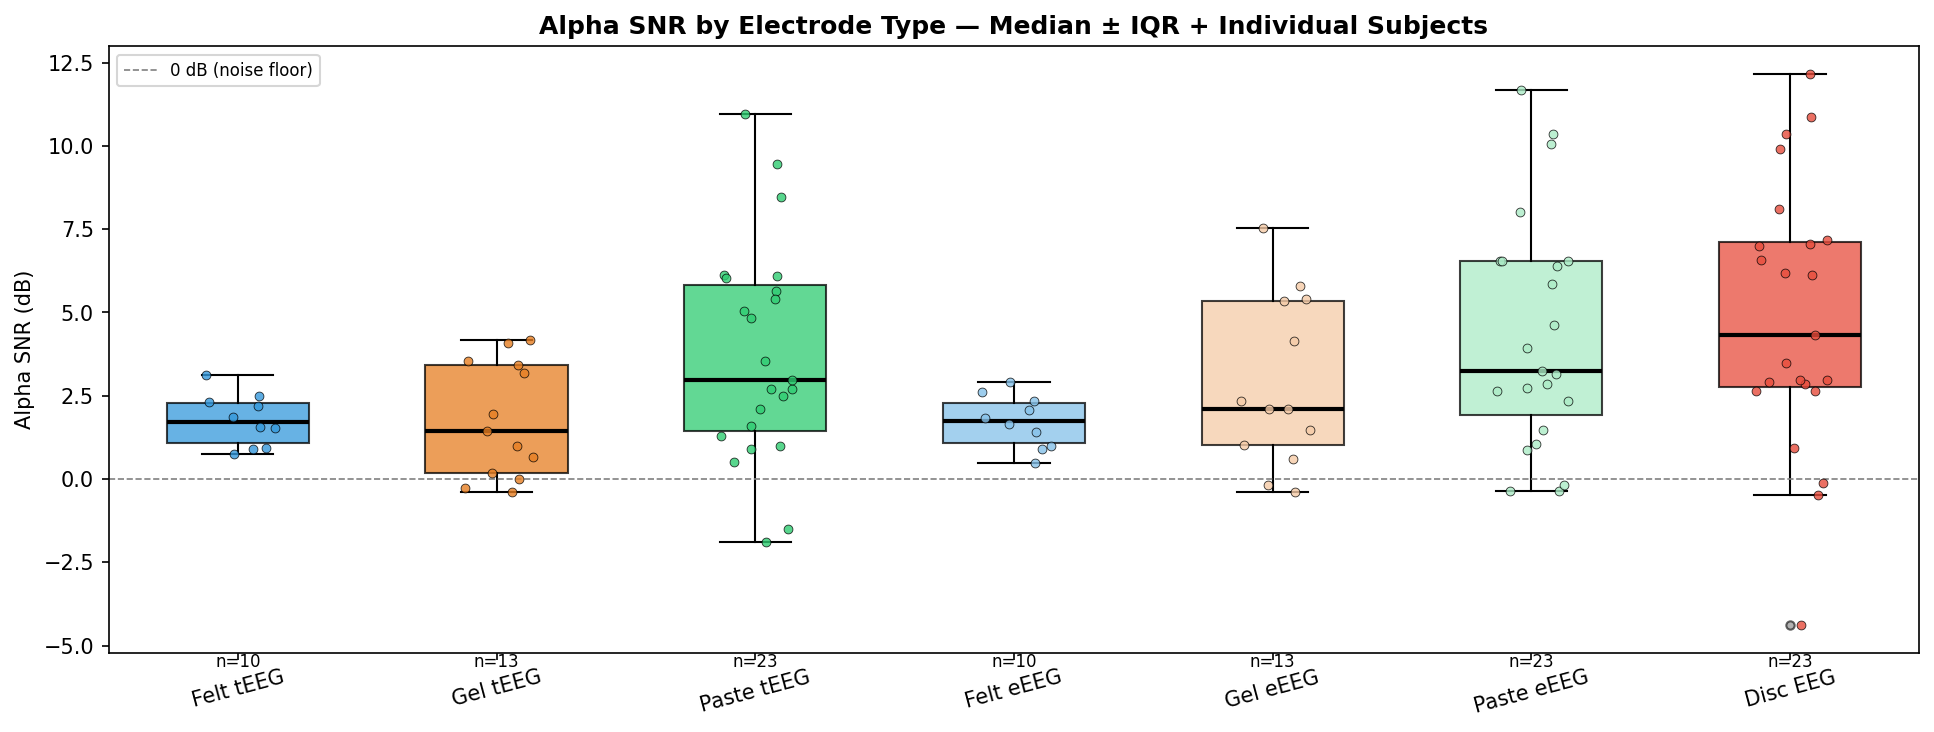
\includegraphics[width=0.95\linewidth]{figs/comparison_alpha_snr.png}
\caption{Alpha-band SNR (dB) by electrode class. Boxplots overlaid with individual-subject points. $n$ = subjects per class.}
\label{fig:alpha_snr}
\end{figure}

\subsection{Eyes-Closed/Eyes-Open Reactivity}
Figure~\ref{fig:reactivity} shows alpha reactivity (closed/open ratio). Values $>1$ indicate the Berger effect~\cite{kirschfeld2005}. Per-class median (BCa 95\% CI): Felt tEEG $1.49$ $[1.10,\ 1.87]$ ($n=10$); Gel tEEG $3.63$ $[1.64,\ 5.32]$ ($n=13$); Paste tEEG $3.43$ $[2.30,\ 6.88]$ ($n=23$); Disc $4.72$ $[2.41,\ 8.62]$ ($n=23$). The Berger effect (reactivity $>1$) is detected on Felt tEEG in 10/10 subjects, Gel tEEG in 13/13, and Paste tEEG in 21/23. Between-setup (Mann--Whitney U) Felt-tEEG vs Gel-tEEG: $U=26$, $p=0.017$, $d=-1.11$ --- gel reactivity exceeds felt reactivity by a notable margin. Within-setup paired (Wilcoxon signed-rank) Felt-tEEG vs Paste-tEEG: $W=5$, $p=0.020$, $d_z=-0.58$ ($n_{\mathrm{pairs}}=10$); Gel-tEEG vs Paste-tEEG: $W=23$, $p=0.13$, $d_z=-0.43$ ($n_{\mathrm{pairs}}=13$).

The two paste-tEEG subjects with reactivity $\leq 1$ are SF02 (paste-tEEG reactivity 0.96; disc 5.00; felt-tEEG 1.67) and SF03 (paste-tEEG reactivity 0.88; disc 0.96; felt-tEEG 1.10). For SF03 the attenuated Berger response is consistent across all three derivations and reads as a subject-level effect. For SF02 the non-response is confined to the paste-tEEG channel while disc and felt-tEEG channels show the expected modulation, which is more consistent with a placement-level issue on the paste TCRE during that session; SF02 also carries a $3.3\%$ ADC-clip WARN flag (Table~\ref{tab:qc}). We retain both subjects in the cohort and flag the non-response transparently rather than dropping them.

The Felt-tEEG reactivity median (1.49) is notably lower than the Gel-tEEG median (3.63). Three non-exclusive factors plausibly contribute. (i) ADC clipping is concentrated in the felt cohort: four of ten felt sessions (LF02, SF01, SF02, SF07; Table~\ref{tab:qc}) carry a clip-percentage WARN flag, and the rail-clipping event most commonly occurs on high-amplitude eyes-closed segments where it depresses measured $P_{\alpha,\mathrm{closed}}$. (ii) The eyes-closed/eyes-open epoch counts are smaller in the felt cohort (median 4 / 3 epochs vs.\ median 3 / 3 in the gel cohort, with the gel cohort sometimes recording only $2/2$), and the closed-condition power estimate is correspondingly noisier on a per-subject basis. (iii) A residual construction effect cannot be excluded: saline coupling may attenuate posterior alpha at the scalp through its broader and lower-impedance footprint. We retain the Felt-tEEG cohort in the main analysis because the Berger effect (reactivity $>1$) is detected in 10/10 felt subjects, but read the absolute reactivity \emph{magnitude} as confounded with acquisition quality and not as a clean construction-level number.

\begin{figure}[H]
\centering
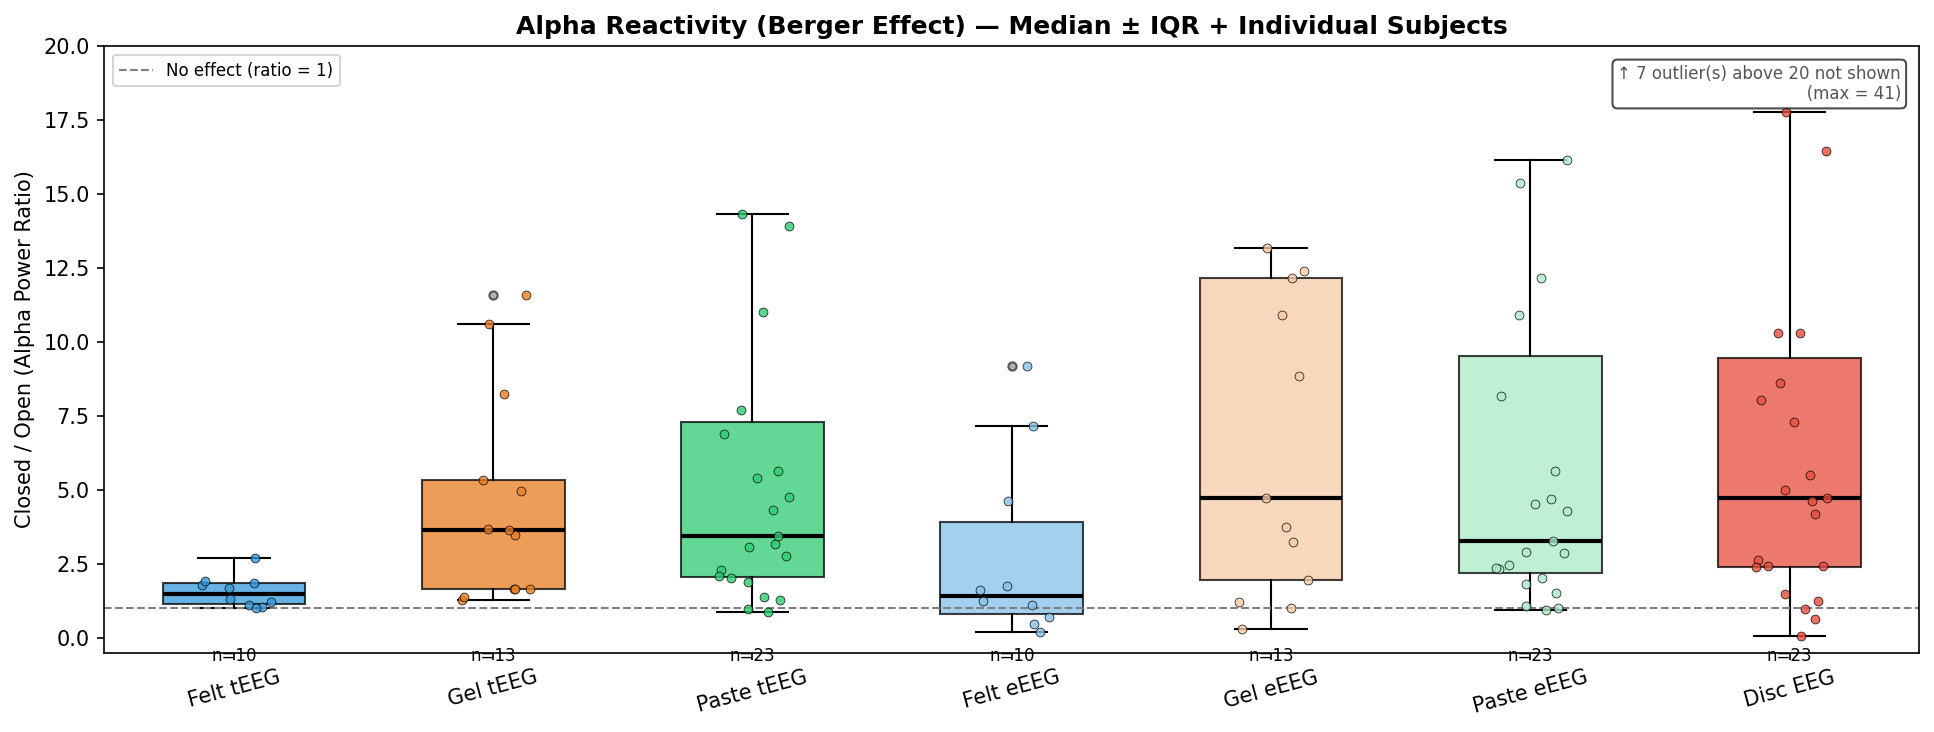
\includegraphics[width=0.95\linewidth]{figs/comparison_alpha_reactivity.png}
\caption{Alpha reactivity (eyes-closed/eyes-open alpha power) by electrode class. Reactivity axis is capped, with outliers annotated.}
\label{fig:reactivity}
\end{figure}

\subsection{Eyes-Open versus Eyes-Closed PSD Shape}
Figure~\ref{fig:open_closed_psd} shows the per-class normalized PSDs for eyes-open and eyes-closed. PSDs are normalized to each channel's own broadband power (1--30~Hz) so that shape, not amplitude, is compared across constructions.

\begin{figure}[H]
\centering
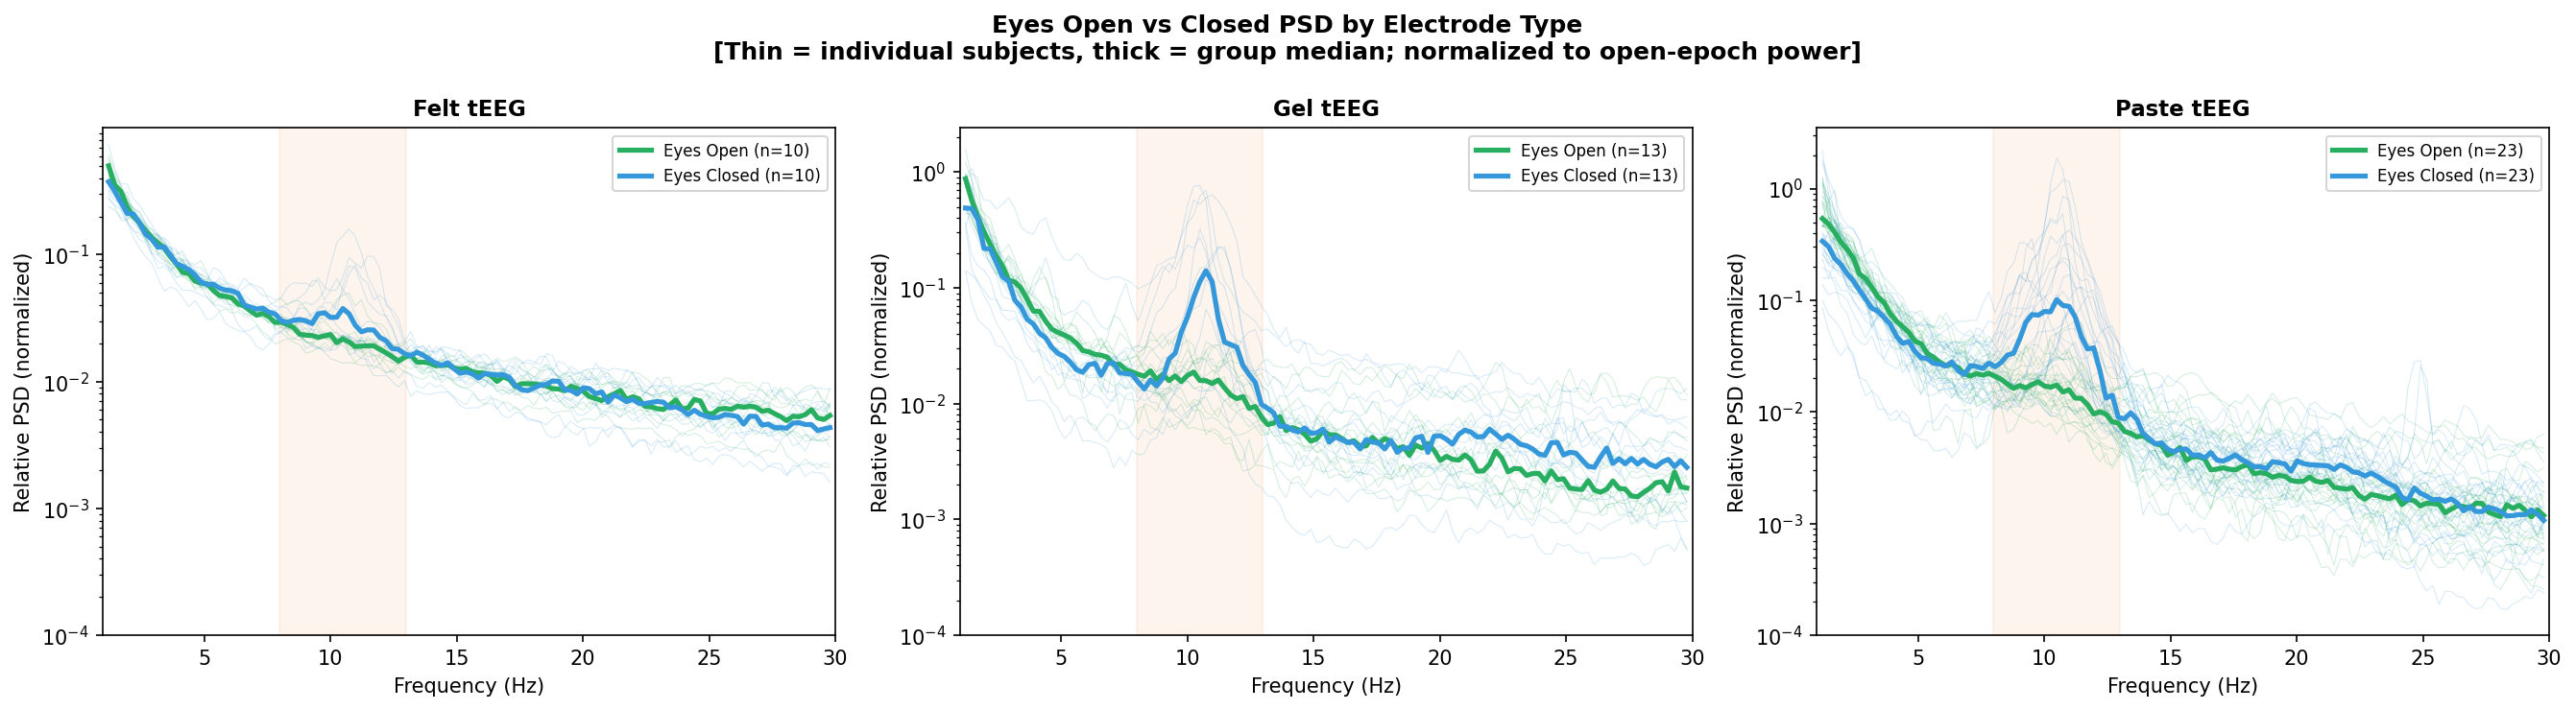
\includegraphics[width=0.95\linewidth]{figs/comparison_open_vs_closed_psd.png}
\caption{Normalized eyes-open vs.\ eyes-closed PSD, per electrode class. An 8--13~Hz bump on closed minus open is the expected Berger signature.}
\label{fig:open_closed_psd}
\end{figure}

\begin{figure}[H]
\centering
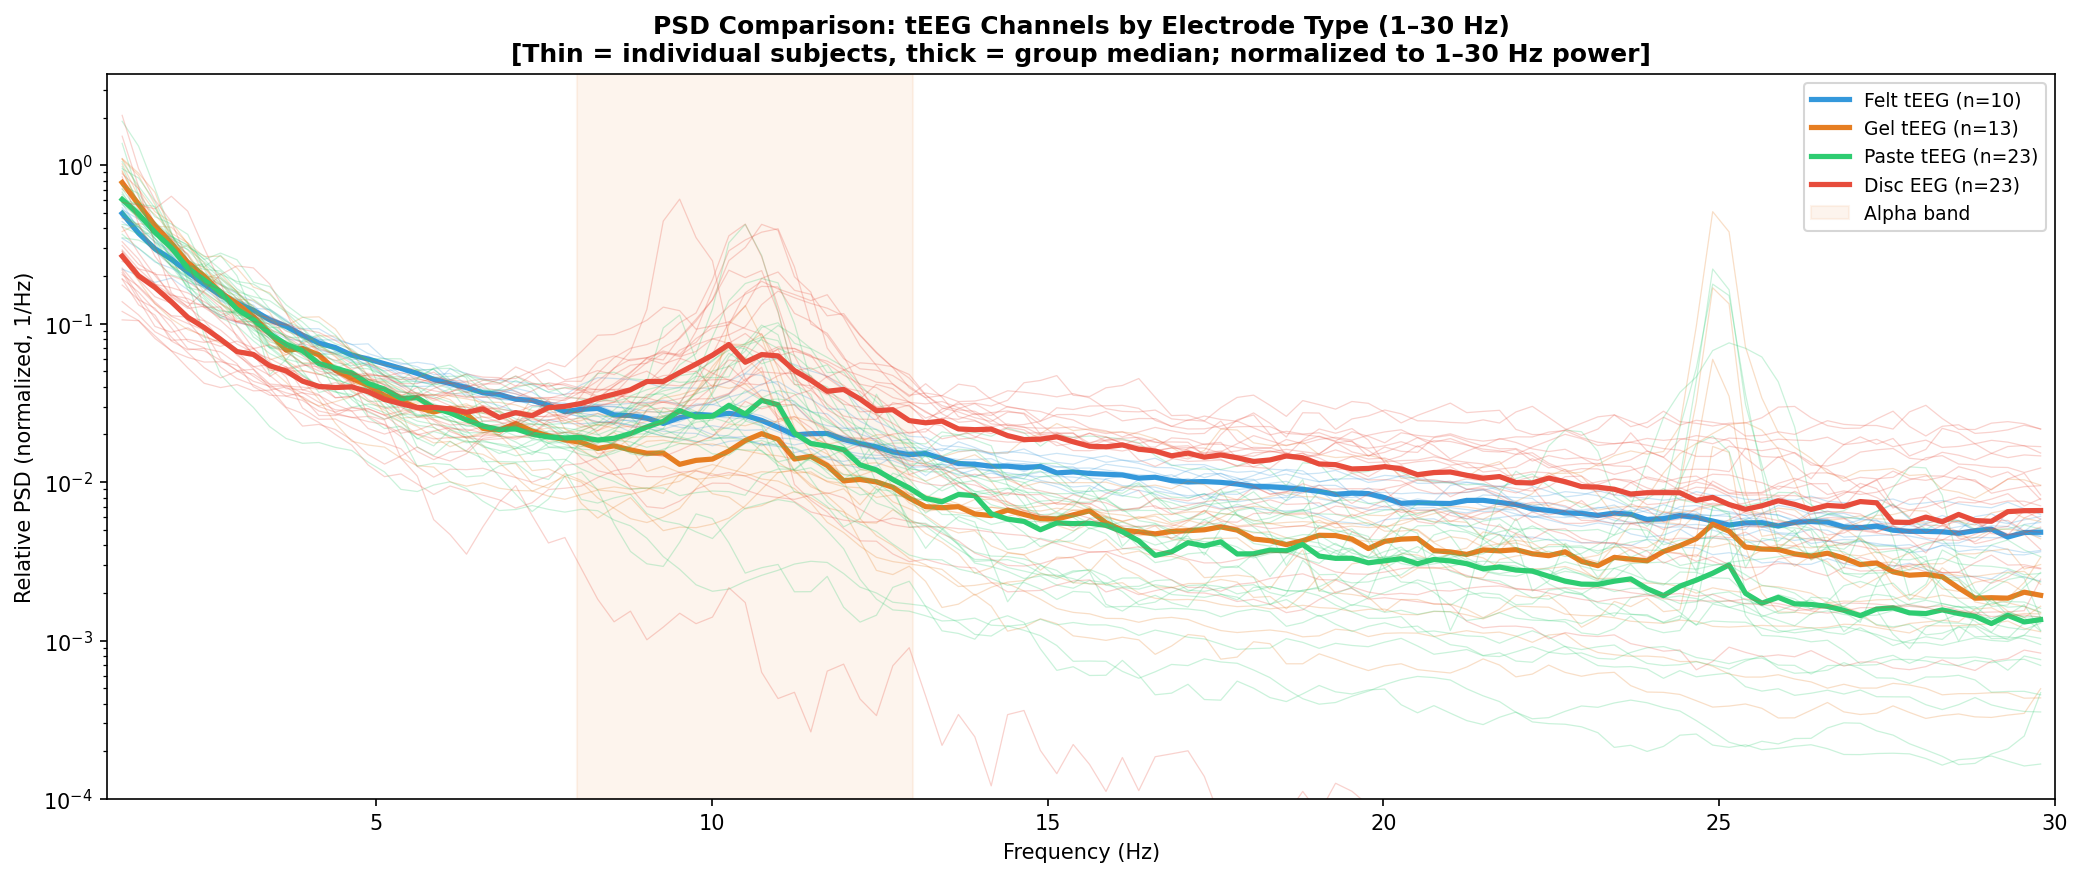
\includegraphics[width=0.95\linewidth]{figs/comparison_psd_teeg.png}
\caption{Normalized tEEG PSDs (1--30~Hz) by electrode class, with the disc reference overlaid. Per-channel broadband normalization makes the shapes directly comparable across constructions.}
\label{fig:psd_teeg}
\end{figure}

\subsection{Spectrogram SSIM Between Paired tEEG and eEEG}
Figure~\ref{fig:ssim} reports the per-pair SSIM between tEEG and eEEG spectrograms. SSIM is bounded in $[0,1]$ and is dimensionless, so values are directly comparable across the two acquisition setups. Per-class median (BCa 95\% CI): Felt $0.307$ $[0.266,\ 0.338]$ ($n=10$); Gel $0.519$ $[0.470,\ 0.694]$ ($n=13$); Paste $0.710$ $[0.619,\ 0.758]$ ($n=23$). All three constructions cluster well below the 0.8 conventional ``high-similarity'' threshold, supporting the interpretation that tEEG and eEEG are not simply scaled copies of each other. The construction effect on tEEG--eEEG SSIM is strong across the cohort: between-setup, Felt-tEEG vs Gel-tEEG differs at $U=0$, $p<0.001$, $d=-2.52$ ($n_a=10$, $n_b=13$, Mann--Whitney). Within-setup paired contrasts (Wilcoxon signed-rank) confirm the same ordering: Felt vs Paste, $W=1$, $p=0.004$, $d_z=-1.95$ ($n_{\mathrm{pairs}}=10$); Gel vs Paste, $W=7$, $p=0.005$, $d_z=-1.03$ ($n_{\mathrm{pairs}}=13$). The ordering Felt $<$ Gel $<$ Paste is consistent across all three contrasts.

\begin{figure}[H]
\centering
\IfFileExists{figs/comparison_ssim.png}{%
  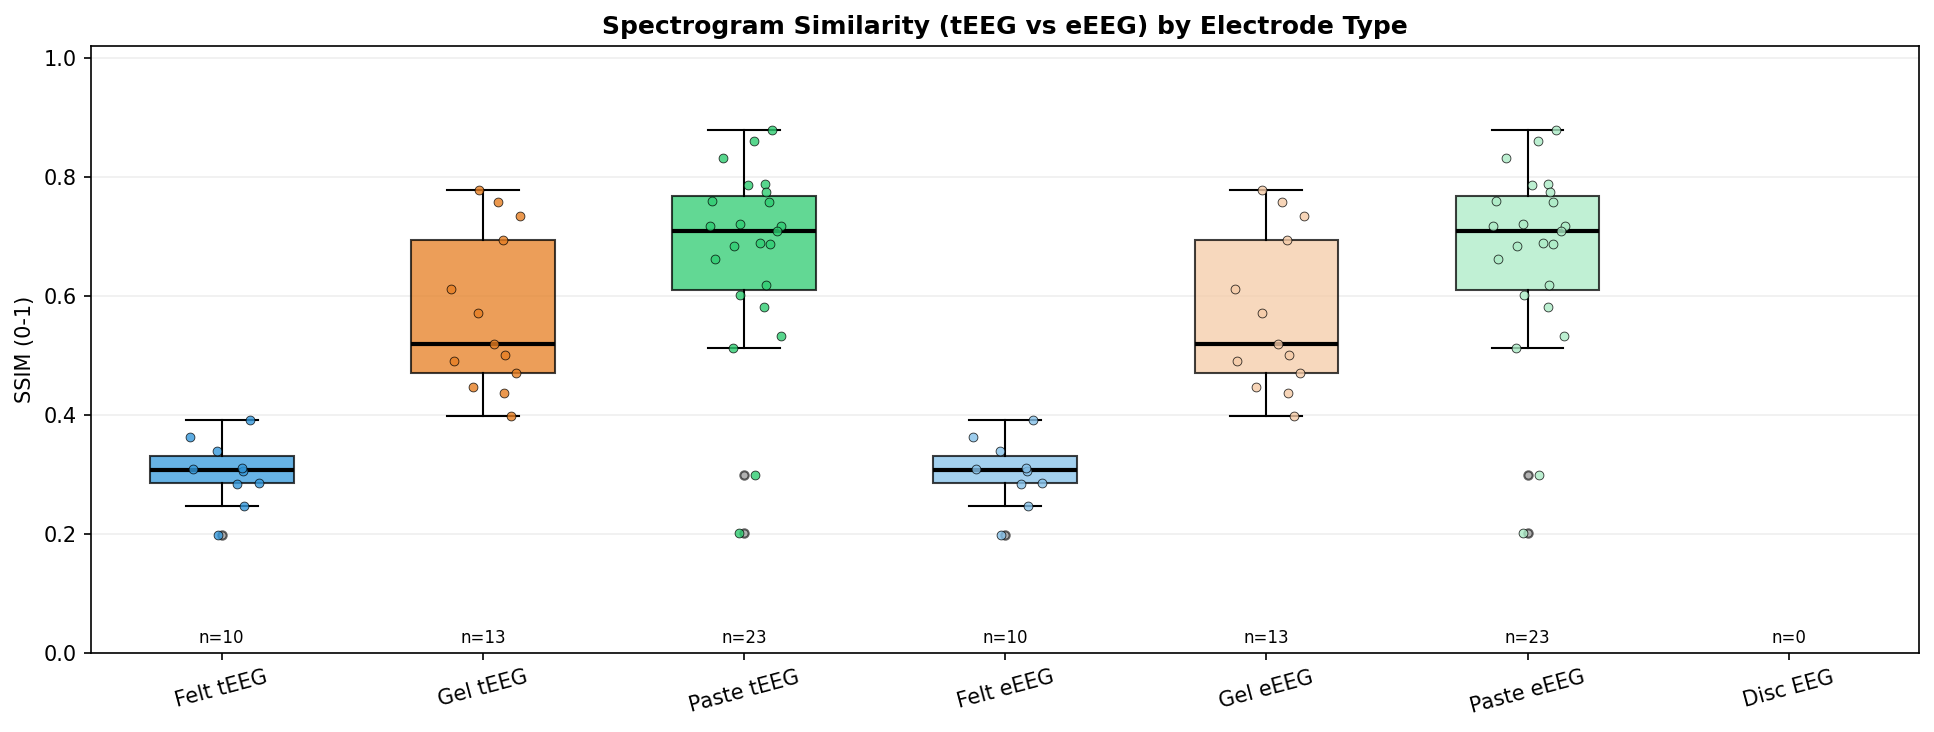
\includegraphics[width=0.95\linewidth]{figs/comparison_ssim.png}%
}{%
  \fbox{\parbox{0.7\linewidth}{\centering\vspace{1.5em}\textit{[comparison\_ssim.png missing --- re-run \texttt{src/three\_way\_comparison.ipynb}]}\vspace{1.5em}}}%
}
\caption{Spectrogram SSIM between paired tEEG and eEEG channels by electrode class.}
\label{fig:ssim}
\end{figure}

\subsection{Paste-TCRE Cross-Setup Bridge}
Because the paste TCRE is present in both setups, between-setup differences in its behavior estimate the residual cross-setup variance not attributable to construction. Figure~\ref{fig:paste_bridge} shows paste-TCRE metrics in the felt setup vs.\ the gel setup. None of the three Mann--Whitney comparisons reach significance (alpha SNR: $U=89$, $p=0.15$, $d=+0.51$; reactivity: $U=46$, $p=0.25$, $d=-0.39$; SSIM: $U=69$, $p=0.83$, $d=+0.01$; $n_{\mathrm{felt}}=10$, $n_{\mathrm{gel}}=13$). With these sample sizes the bridge has approximately 60\% power to detect a Cohen's $d$ of $0.8$ at $\alpha=0.05$; smaller between-setup effects cannot be ruled out. The point estimates do not, however, reproduce the magnitude or direction of the cross-construction contrasts in §\ref{sec:cohort_qc}--§3.5 (most notably the very large Felt vs Gel SSIM effect of $d=-2.52$), which supports the interpretation that the construction-level effects reported here are not driven primarily by between-setup acquisition differences.

\begin{figure}[H]
\centering
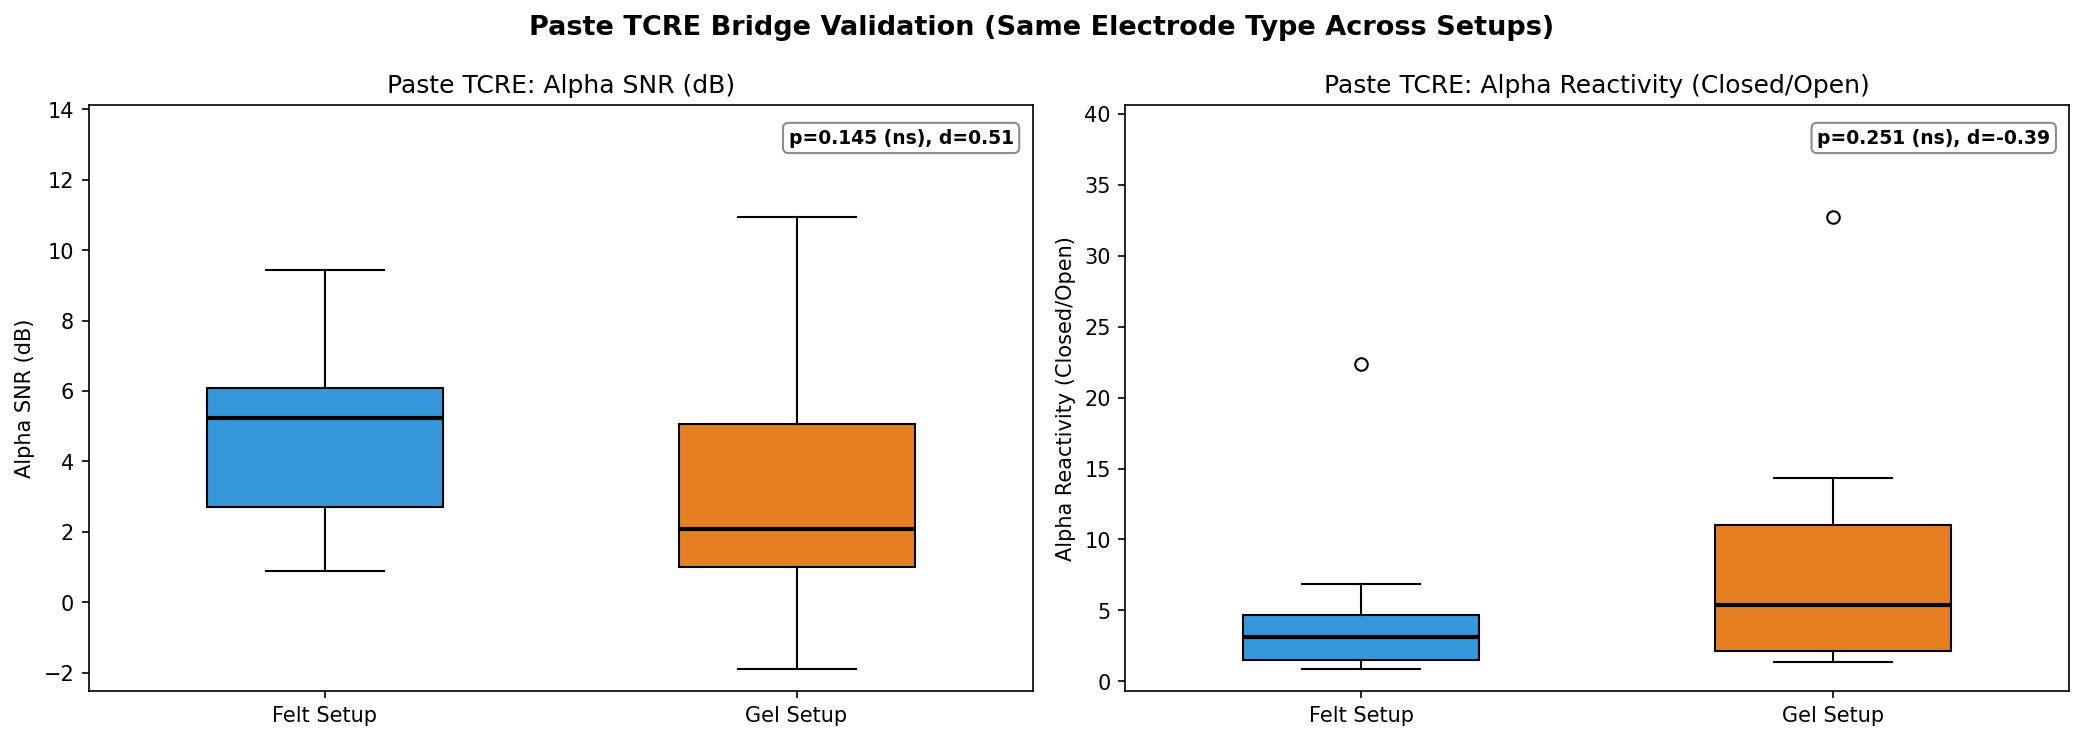
\includegraphics[width=0.95\linewidth]{figs/comparison_paste_bridge.png}
\caption{Paste TCRE behavior in the felt setup vs.\ the gel setup (cross-setup bridge). Endpoints: alpha SNR, reactivity, and SSIM.}
\label{fig:paste_bridge}
\end{figure}

\subsection{Visual Evoked Potentials (Felt Setup Only)}\label{sec:vep_scope}
VEPs are reported as a qualitative check on the felt setup; the section is intentionally limited to the two long-felt subjects whose pre-averaged checkerboard responses are available (LF02 and LF03). Figure~\ref{fig:felt_vep} shows the per-subject grand averages over the felt-tEEG (channel-mean of TCRE \#1--\#4 tEEG), paste-tEEG, and paste-disc derivations, with N75 / P100 / N135 markers placed at the canonical-window extrema (Table~\ref{tab:felt_vep}). The cleanest morphology in the cohort is on LF02 paste-tEEG, with a resolved P100 at 109~ms ($\approx 17\ \upmu$V) flanked by a 71~ms N75 and a 132~ms N135; the disc on the same subject produces a small but matching deflection. On LF03 the paste-tEEG channel shows a large positive deflection at $\approx 41\ \upmu$V near 140~ms, but because this latency is at the upper boundary of the canonical P100 window we do not report it as a resolved P100; the broader morphology suggests a delayed or atypically-shaped positivity that is more compatible with a P100/N135 fusion than with a textbook P100. LF02 felt-tEEG amplitudes are noise-dominated because the felt-tEEG channel mean is contaminated by the clipping flagged in Table~\ref{tab:qc}; we retain the row in Table~\ref{tab:felt_vep} for transparency only. Peak-finding here is the simple within-window extremum search documented in \texttt{scripts/build\_felt\_vep\_figure.py}; latencies that would otherwise pin at a window boundary (50, 125, or 140~ms) are reported as ``n.r.'' (not resolved) rather than as numerical peaks. With $n=2$ usable VEP recordings, this section is hypothesis-generating and should not be read as a quantitative VEP comparison; an expanded VEP cohort under the harmonized pipeline is left for future work.

The gel cohort is excluded from cross-construction VEP statistics because the gel-era acquisition produced unreliable evoked responses when re-processed under the harmonized pipeline. We document the gel-VEP behaviour qualitatively in Section~\ref{sec:gel_vep_sanity} so that the exclusion is auditable; the underlying cause (amplifier configuration during the gel collection campaign vs.\ residual pipeline differences) is currently under review with the original gel-TCRE operator.

\begin{figure}[H]
\centering
\IfFileExists{figs/felt_vep_grand.png}{%
  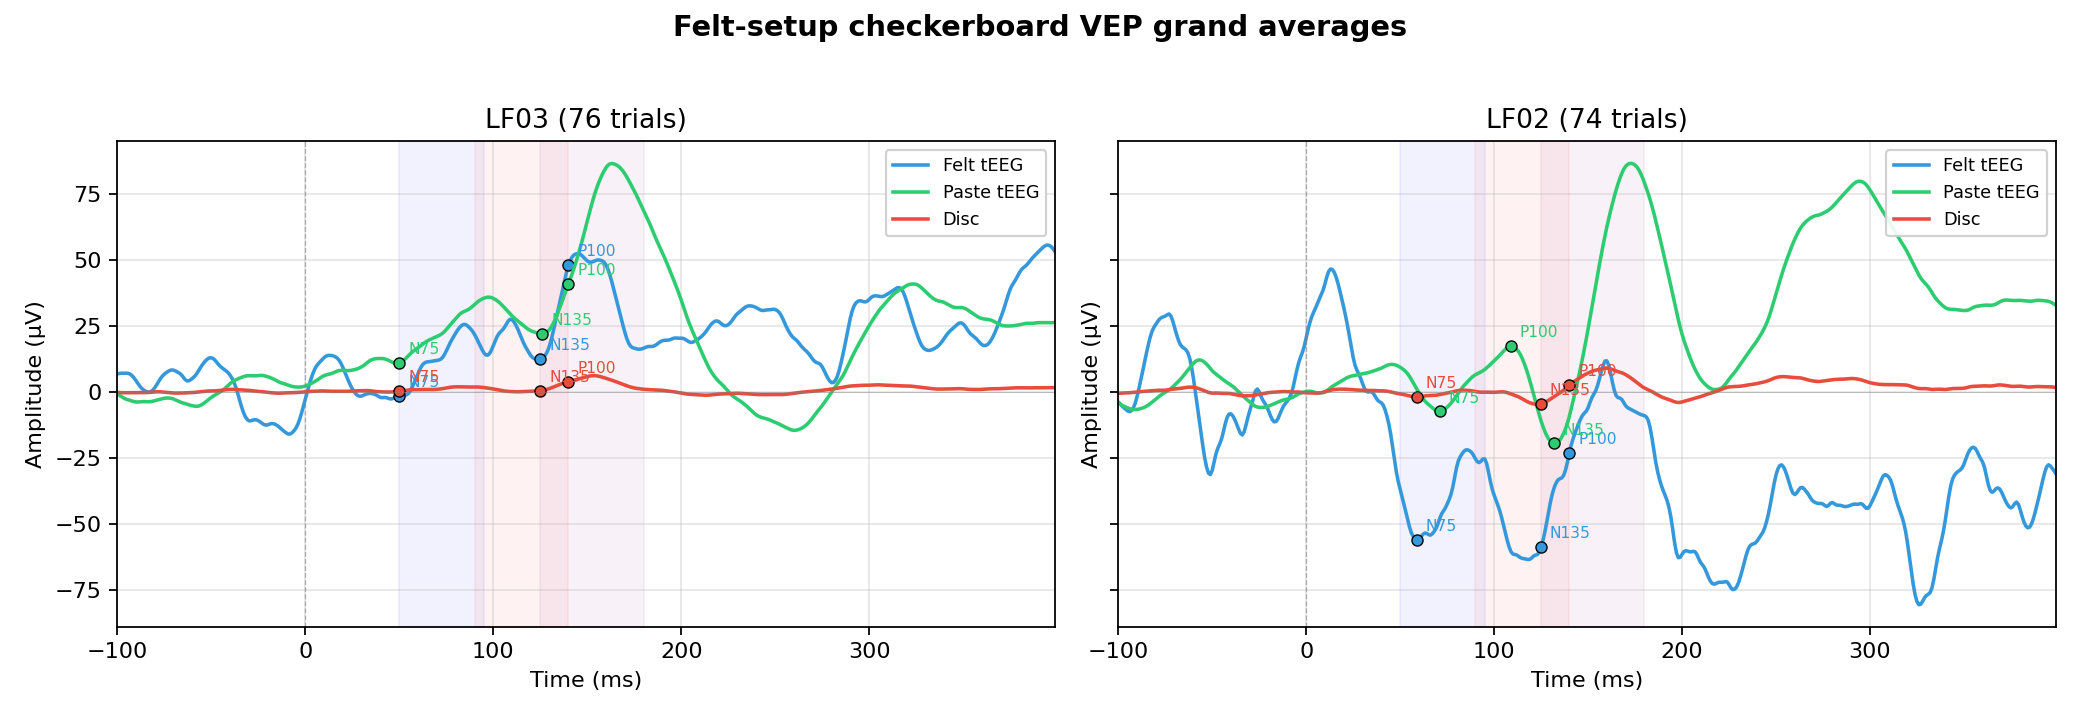
\includegraphics[width=0.95\linewidth]{figs/felt_vep_grand.png}%
}{%
  \fbox{\parbox{0.7\linewidth}{\centering\vspace{1.5em}\textit{[felt\_vep\_grand.png missing --- run \texttt{python paper\_sensors/build\_felt\_vep\_figure.py}]}\vspace{1.5em}}}%
}
\caption{Felt-setup checkerboard VEP grand averages for subjects LF02 and LF03 (mean over tEEG channels of the four felt TCREs; paste-TCRE \#5 tEEG; paste disc). Vertical dashed line: stimulus onset. Coloured bands: N75 (blue), P100 (red), N135 (purple) search windows.}
\label{fig:felt_vep}
\end{figure}

\begin{table}[H]
\caption{Per-subject VEP latencies (ms) and amplitudes ($\upmu$V) on the felt-tEEG channel-mean, paste-tEEG, and disc. Subject IDs follow the de-identified codes in Table~\ref{tab:qc}. Latencies that would otherwise pin at a canonical-window boundary (50, 140, or 125~ms) are reported as ``n.r.'' (not resolved) because they indicate the peak-finder returned the within-window extremum rather than a true local extremum. The LF02 felt-tEEG row is shown in grey because the felt-tEEG mean on that subject is dominated by a clipped/high-impedance channel (Table~\ref{tab:qc}) and the values are noise-dominated; we retain the row for transparency rather than for interpretation. Resolved peaks are reported numerically.}
\label{tab:felt_vep}
\centering\small
\begin{tabular}{llcccccc}
\toprule
\textbf{ID} & \textbf{Channel} & \textbf{N75 lat} & \textbf{N75 amp} & \textbf{P100 lat} & \textbf{P100 amp} & \textbf{N135 lat} & \textbf{N135 amp} \\
\midrule
LF03 & Felt tEEG  & n.r.\ & $-1.7$  & n.r.\ & $+48.0$ & n.r.\ & $+12.5$ \\
LF03 & Paste tEEG & n.r.\ & $+10.9$ & n.r.\ & $+41.0$ & 126.0 & $+22.1$ \\
LF03 & Disc       & n.r.\ & $+0.2$  & n.r.\ & $+3.9$  & n.r.\ & $+0.4$  \\
\midrule
LF02 & Felt tEEG\footnotemark[1] & 59.0 & $-56.0$ & n.r.\ & $-23.3$ & n.r.\ & $-59.0$ \\
LF02 & Paste tEEG & 71.0  & $-7.4$  & 109.0 & $+17.3$ & 132.0 & $-19.6$ \\
LF02 & Disc       & 59.0  & $-1.9$  & n.r.\ & $+2.6$  & n.r.\ & $-4.5$  \\
\bottomrule
\end{tabular}
\par\smallskip
\footnotetext[1]{LF02 felt-tEEG values are noise-dominated because the felt-tEEG mean is contaminated by the clipped channel flagged in Table~\ref{tab:qc}; reported for transparency only.}
\end{table}

\subsection{Gel-Cohort VEP Sanity Check (Qualitative)}\label{sec:gel_vep_sanity}
Three gel-cohort recordings illustrate the heterogeneity behind the cross-construction VEP exclusion: G02 and G10 (both in the analysis cohort) and one additional gel session that failed cohort QC due to continuous ADC-rail saturation on its tEEG channel (referred to here as the excluded session). Recognisable VEP morphology (N75/P100/N135) is recoverable on at least one tEEG channel for G02 (marginal) and G10 (clearest, with matching morphology on the paired Pz disc at smaller amplitude); the excluded session's tEEG saturates the INT16 rail, while its paired disc still produces a recognisable VEP (Figures~\ref{fig:gel_vep_ba1}--\ref{fig:gel_vep_mn3}). A short preprocessing-sensitivity check on the excluded session across the A/B/C variants is shown in Figure~\ref{fig:gel_vep_sensitivity}, and a unified-pipeline overview across the three sessions is shown in Figure~\ref{fig:gel_vep_unified}. The gel-cohort VEPs are not categorically absent under the harmonized pipeline but are not yet of a quality that supports cross-construction VEP statistics.

\begin{figure}[H]
\centering
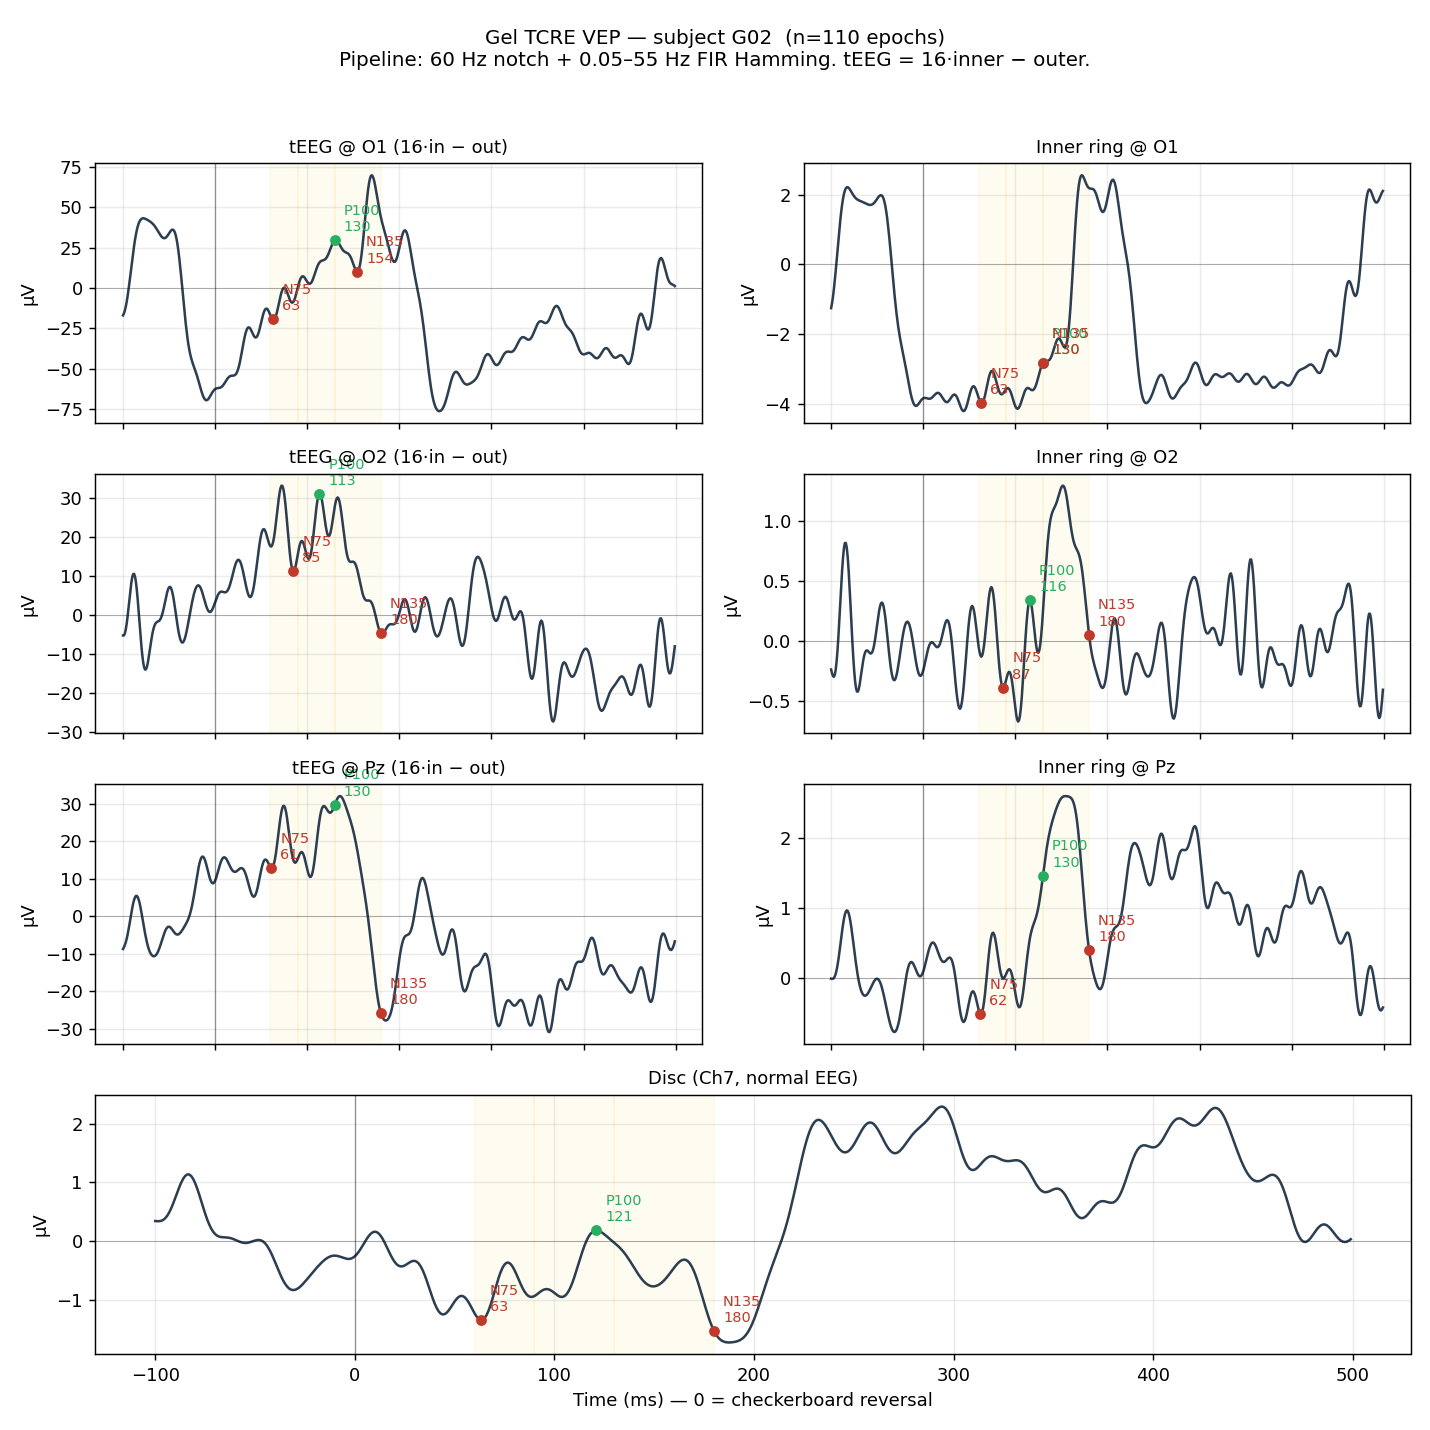
\includegraphics[width=0.95\linewidth]{figs/gel_vep_G02.png}
\caption{Gel-cohort VEP sanity check, subject G02, harmonized pipeline.}
\label{fig:gel_vep_ba1}
\end{figure}

\begin{figure}[H]
\centering
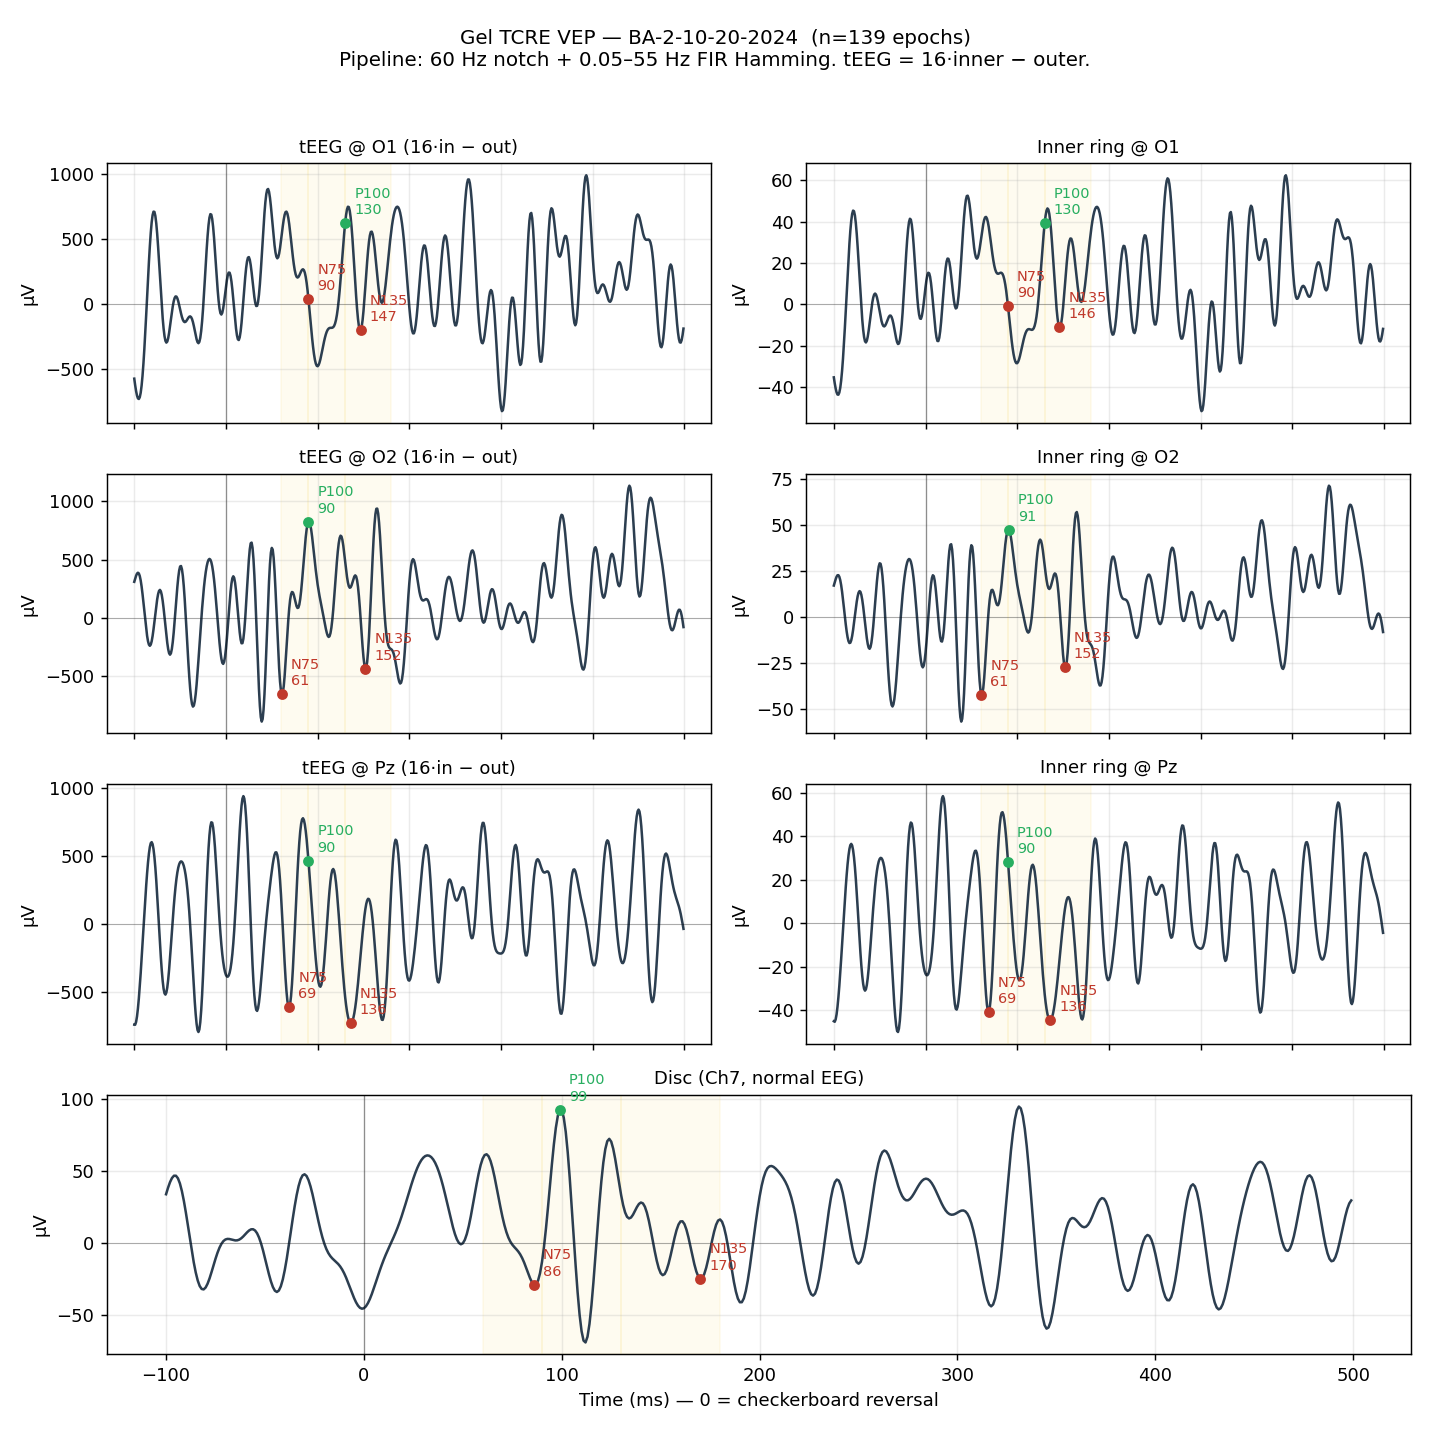
\includegraphics[width=0.95\linewidth]{figs/gel_vep_excluded.png}
\caption{Gel-cohort VEP sanity check, the excluded gel session. The tEEG channel hits the INT16 ADC rail (continuous saturation, QC fail); the paired Pz disc still produces a recognisable evoked response.}
\label{fig:gel_vep_ba2}
\end{figure}

\begin{figure}[H]
\centering
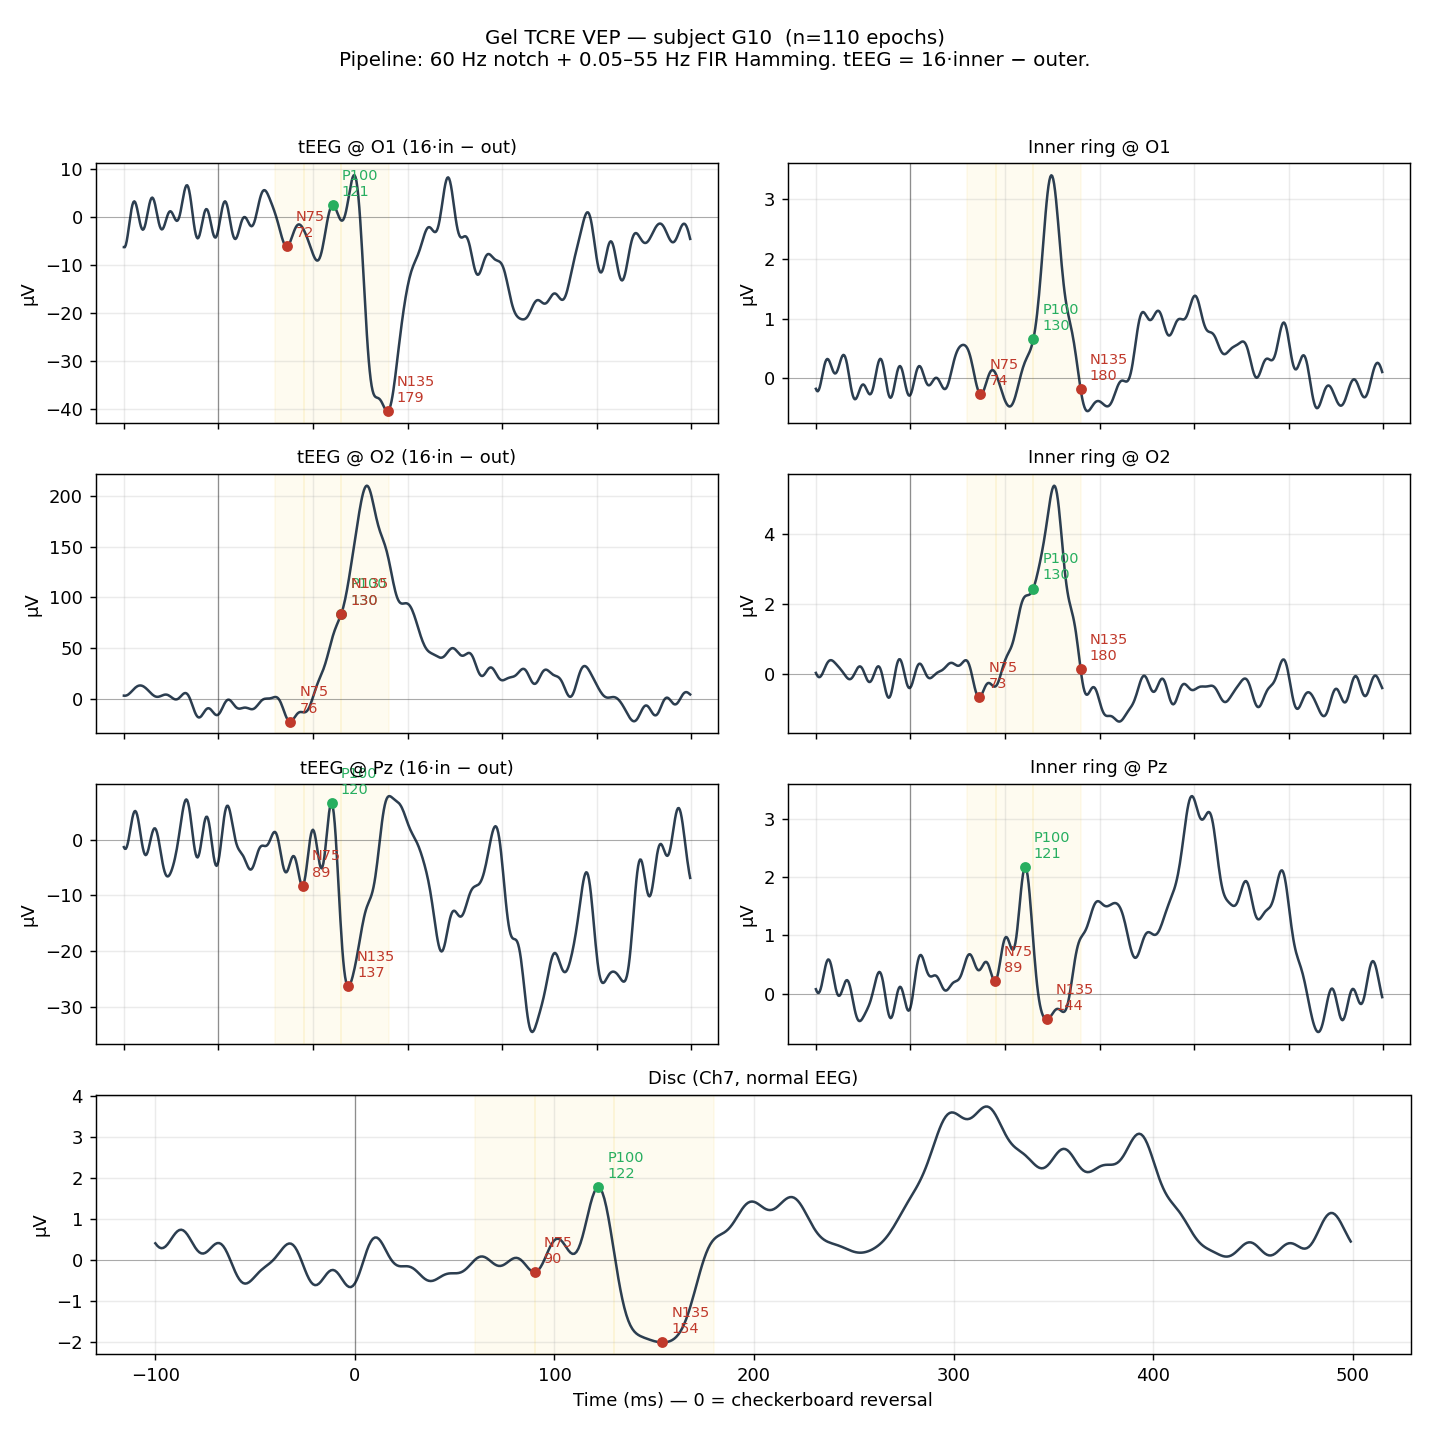
\includegraphics[width=0.95\linewidth]{figs/gel_vep_G10.png}
\caption{Gel-cohort VEP sanity check, subject G10. Cleanest of the three sessions, with N75/P100/N135 visible on tEEG at Pz and matching morphology on the paired Pz disc at smaller amplitude.}
\label{fig:gel_vep_mn3}
\end{figure}

\begin{figure}[H]
\centering
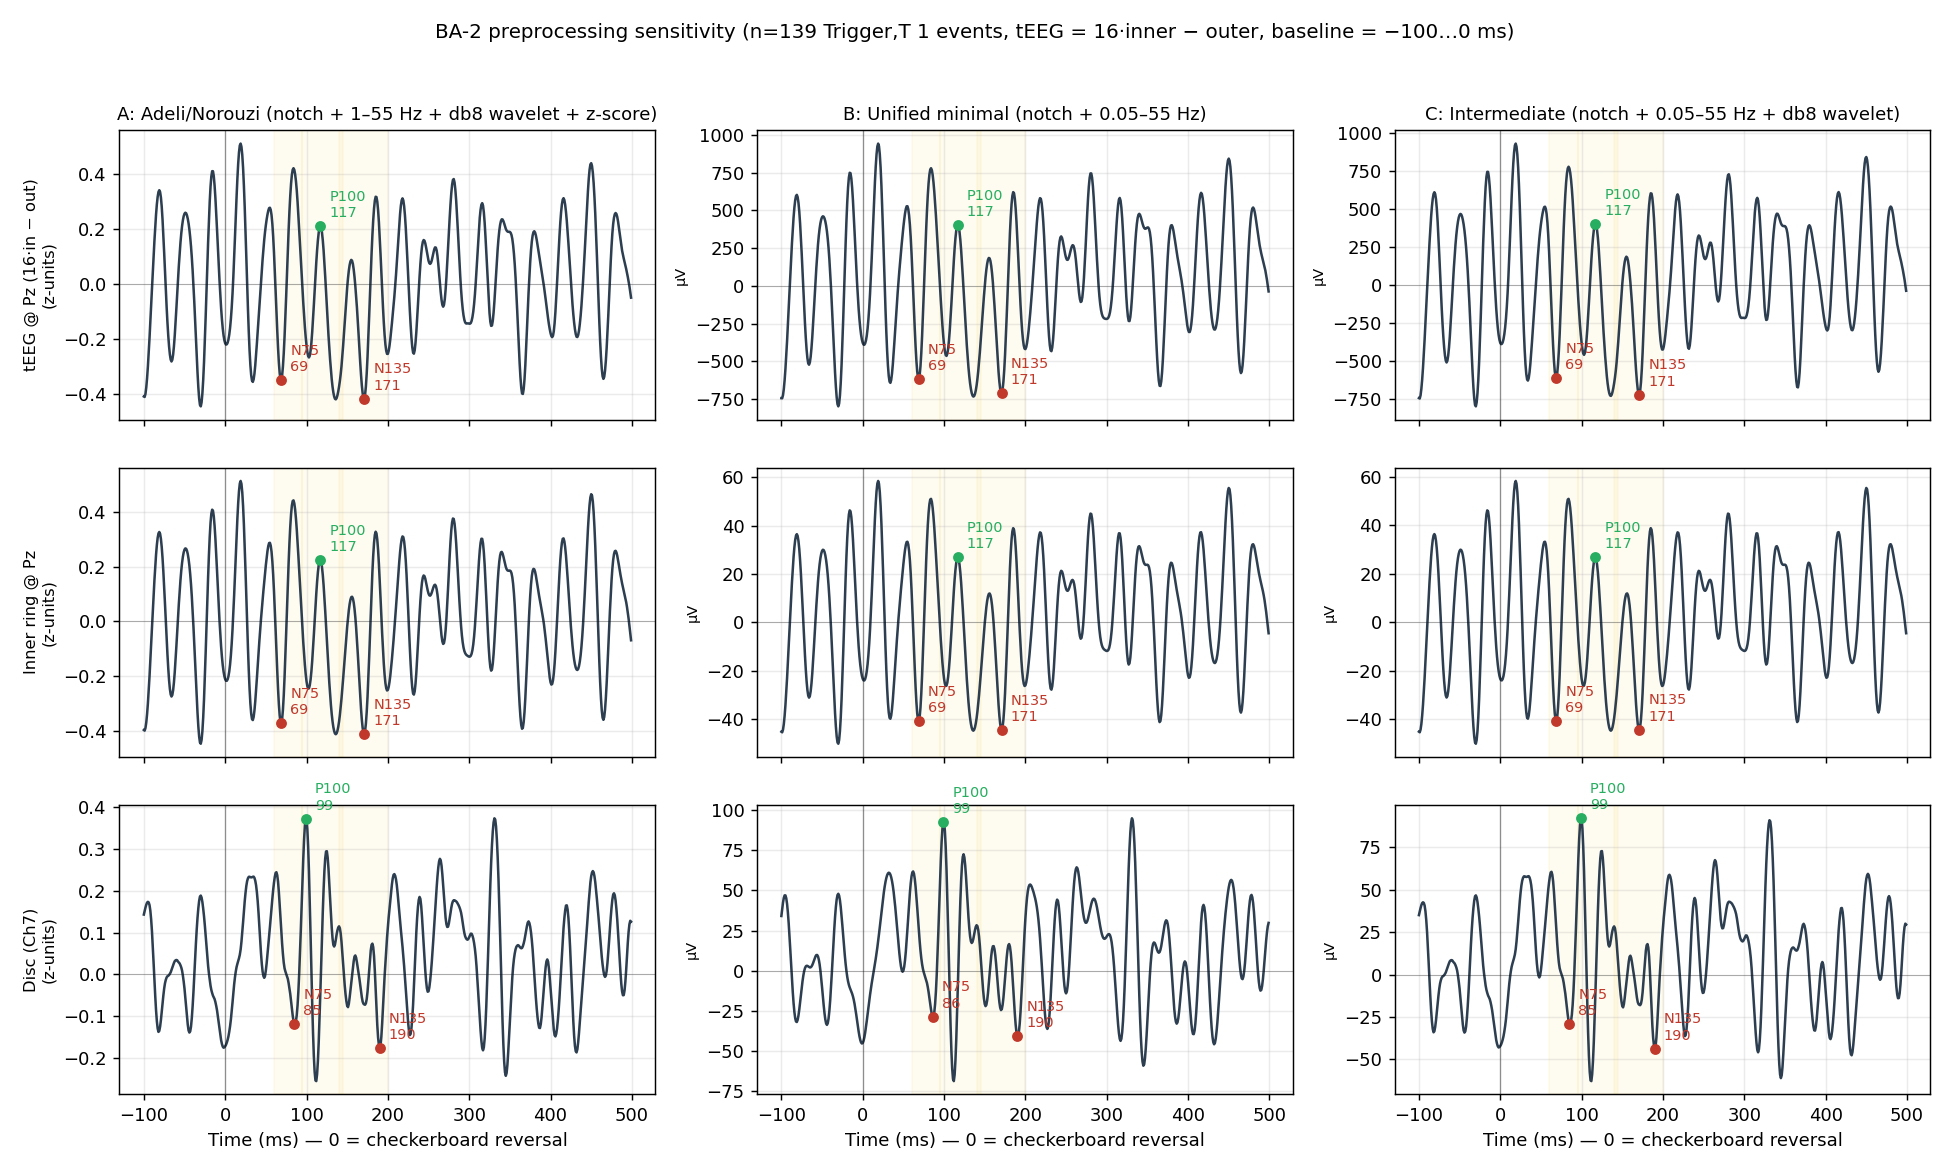
\includegraphics[width=0.95\linewidth]{figs/gel_vep_excluded_sensitivity.png}
\caption{Preprocessing-sensitivity check on the excluded gel session across pipeline variants A (notch + bandpass + wavelet + per-epoch z-score), B (notch + bandpass; primary), and C (notch only). The tEEG ADC saturation persists across all variants, indicating an acquisition-side rather than processing-side cause.}
\label{fig:gel_vep_sensitivity}
\end{figure}

\begin{figure}[H]
\centering
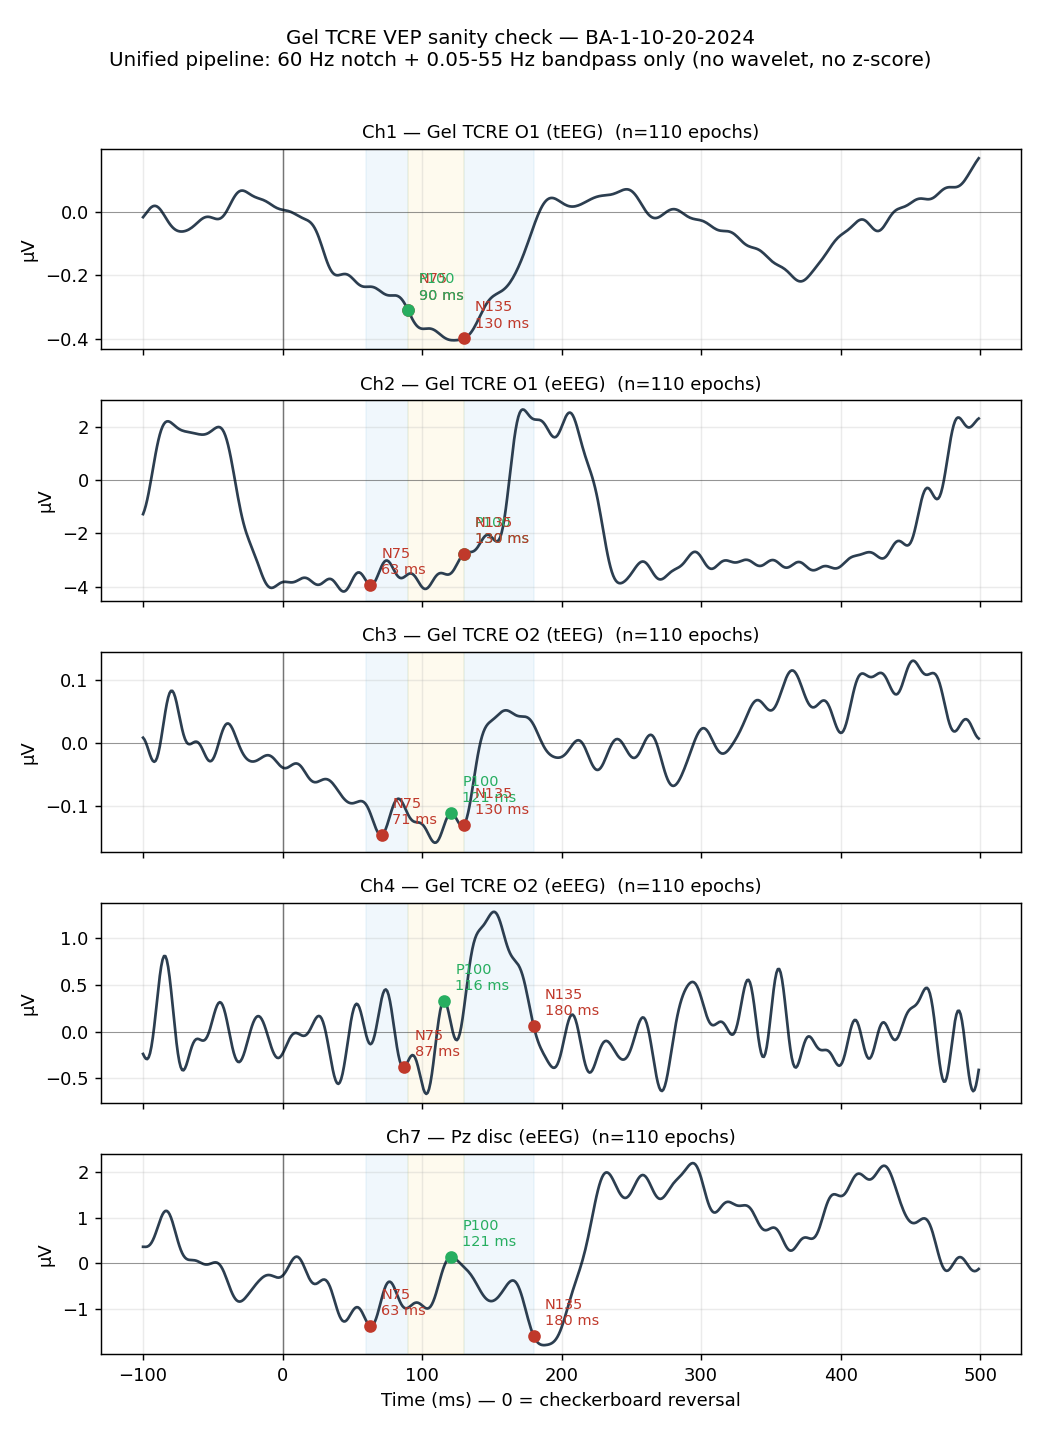
\includegraphics[width=0.95\linewidth]{figs/gel_vep_unified.png}
\caption{Unified-pipeline overview across the gel BA subjects.}
\label{fig:gel_vep_unified}
\end{figure}

%-------------------------------------------------------------------------------
\section{Discussion}

\subsection{Methods Harmonization}
The strongest contribution of this pilot is the harmonized pipeline itself. By excluding adaptive cleaners (ICA, ASR, automated bad-channel interpolation) and keeping the only mandatory steps a notch and a linear-phase bandpass, we ensure that any between-construction differences are not artifacts of a cleaner behaving differently on clean paste vs.\ noisier felt. The cost of this choice is that subjects with bad channels stay flagged rather than rescued, which we report transparently in QC.

\subsection{Felt-tEEG vs.\ Gel-tEEG: Same Estimator, Same Geometry}
Both setups use the same hardware Laplacian on TCREs of identical ring geometry, so the cross-construction contrast in §3 is on construction (electrolyte and coupling: saline-soaked felt vs.\ conductive gel vs.\ paste) rather than on estimator.

A first-pass interpretation of the Felt $<$ Gel $<$ Paste SSIM ordering is that saline coupling produces the largest structural contrast between the Laplacian and conventional derivations recorded on the same TCRE. We note three caveats. First, SSIM is a similarity metric and does not by itself distinguish between two channels carrying genuinely independent neural information and two channels sharing a common neural signal but corrupted by independent noise; lower SSIM is consistent with both. Second, the alpha-SNR ordering (Paste $>$ Felt $\sim$ Gel) does not mirror the SSIM ordering, which argues against a simple ``felt is the cleanest spatial filter'' reading. Third, plausible electrolyte-level mechanisms include differential spreading of saline beyond the nominal ring footprint, effectively enlarging the outer-ring contact area; inter-ring impedance asymmetry, which would inject construction-dependent common-mode-rejection imbalances into the on-board Laplacian; and independent contact-noise contributions to each ring. Direct ring-by-ring impedance logging in future cohorts would discriminate among these. We therefore frame the SSIM ordering as a hypothesis-generating observation about electrolyte coupling rather than as a mechanistic conclusion about which construction provides better spatial filtering.

\subsection{Why Disc-EEG Alpha SNR Exceeds tEEG Alpha SNR}
Disc-EEG alpha SNR (median 4.33~dB) is higher than every tEEG class. The surface Laplacian is expected to improve focal-source detection by suppressing volume-conducted broadband activity~\cite{besio2006,koka2007}, but its action on a non-focal source attenuates the source itself: posterior alpha during the eyes-closed condition is broadly distributed across occipital cortex rather than focal, so a high-pass spatial filter rejects much of it. This is the conventional surface-Laplacian explanation for why an estimator that improves focal-source SNR can simultaneously reduce broadband-alpha SNR; we report the disc--tEEG SNR comparison for context, not as evidence against TCRE.

\subsection{Limitations}

\begin{itemize}
\item Pilot-scale cohort. Felt is $n=10$ (3 long-felt, 7 short-felt) and gel is $n=13$ after QC; any single-subject outlier visibly moves the medians and inferential claims should be read as preliminary.
\item ADC clipping was prevalent on early felt sessions (impedance issues). Per-channel exclusions retain the rest of each affected subject but reduce per-class effective $n$ for some channels.
\item Paste-TCRE recordings in the two setups were collected on different days and likely by different operators. The cross-setup bridge therefore estimates an upper bound on construction effects, not a strict null.
\item VEPs are reported only for the felt setup. The gel-era VEP anomaly is not yet root-caused and is documented qualitatively in the supplement.
\end{itemize}

\subsection{What This Enables}
For practitioners, this paper offers a single open pipeline and a cross-setup bridge design that other TCRE labs can re-use to make their results readable against ours. We deliberately do not recommend one construction over another on the basis of this pilot; the contribution is the comparison framework, not a winner.

%-------------------------------------------------------------------------------
\section{Conclusions}

We presented a pilot, methods-harmonized comparison of three TCRE constructions (saline-soaked felt, conductive gel, paste) using a single minimal preprocessing pipeline and scale-invariant endpoints. Across constructions, alpha-band detection and reactivity were physiologically plausible, the paste-TCRE cross-setup bridge produced no significant between-setup differences ($n_{\mathrm{felt}}=10$, $n_{\mathrm{gel}}=13$), and tEEG vs.\ eEEG spectrograms differed structurally and in a construction-dependent way (median SSIM Felt~$0.31 < $ Gel~$0.52 < $ Paste~$0.71$, with Felt vs Gel and Felt vs Paste both reaching $p\leq 0.002$). Conclusions are descriptive given the small and imbalanced cohort. Future work will (i)~grow both cohorts beyond pilot scale, especially balancing the long-felt arm, and (ii)~re-collect a gel-setup VEP dataset on a single amplifier under the harmonized pipeline.

%-------------------------------------------------------------------------------
\vspace{6pt}

\authorcontributions{Conceptualization, W.G.B.; data curation (felt setup), S.K.; data curation (gel setup) and original gel-TCRE signal-processing pipeline, B.A.; hardware and 3D-printed electrode housings, M.\TBD{Surname}; methodology and harmonized analysis pipeline, S.K.; software, S.K.; formal analysis, S.K.; writing---original draft preparation, S.K.; writing---review and editing, all authors; supervision and project administration, W.G.B. All authors have read and agreed to the published version of the manuscript.}

\funding{\TBD{Funding sources and grant numbers (URI / NIH / NSF as applicable).}}

\institutionalreview{\TBD{IRB protocol number and approving body.}}

\informedconsent{Informed consent was obtained from all subjects involved in the study.}

\dataavailability{Code is available at \TBD{repo URL}. De-identified processed metrics will be released alongside the final manuscript; raw recordings remain access-controlled under the URI IRB protocol.}

\acknowledgments{The authors thank Tugba \TBD{Surname} and Hunter \TBD{Surname} (graduate students, URI Biomedical Engineering, Spring 2026) for assistance with felt-cohort recordings and electrode placement; Luci \TBD{Surname} for designing and 3D-printing the longer screw used in the felt setup and for assistance with recordings; and Caitlin \TBD{Surname} and Gabryana \TBD{Surname} for assistance with recordings. We also thank the subjects who participated and the URI Biomedical Engineering technical staff.}

\conflictsofinterest{The authors declare no conflicts of interest.}

%\sampleavailability{Not applicable.}

%-------------------------------------------------------------------------------
%\reftitle{References}
\begin{adjustwidth}{-\extralength}{0cm}
\printendnotes[custom]
\end{adjustwidth}

\reftitle{References}
\externalbibliography{yes}
\ifpreview\bibliographystyle{unsrt}\fi
\bibliography{refs}

\end{document}
